\section{Upgraded Phase-2 Tracker}

This chapter is dedicated to a study that seeks to optimize the geometry of the Phase-2 Pixel Detector (for the HL-LHC) in terms of how the upgraded Inner Tracker (IT) affects the overall stub production (the concept of a stub is defined in \autoref{stubDefSec}). The goal of this study was to determine how the removal of discs from the Phase-2 Forward Pixel detector would affect the production of L1 stubs in the upgraded CMS Outer Tracker (OT). More information of the Phase-2 Tracker can be found at \cite{Phase2Tracker1}. This study has a direct impact on the future of SUSY analyses due to the importance of the tracker in searches for BSM physics.\\

In the HL-LHC era (2023-2035) an integrated luminosity of 3,000 fb$^{-1}$ is expected to be reached at a center-of-mass energy of 14 TeV. This data will enable us to make precise measurements of several SM parameters (particularly the scalar sector). This will also lay the groundwork for new physics searches proposed by many of the BSM models. In addition, the HL-LHC project is essential to identify any hints of new physics, including SUSY, that could possibly be observed during the LHC Run 2 or 3, or beyond. The bigger, and highly granular pixel and silicon tracker, and its extended $\eta$ coverage, will improve jet sub-structure, boosted object identification and heavy object tagging to hunt for BSM physics, specifically Supersymmetry. A discovery could happen with various few sigma excesses and then interpretation of the new signal will require a large amount of data. At the HL-LHC, much gain is expected for weakly produced SUSY particles because they are characterized by small production cross-sections. Considering the case that gluinos and squarks are heavy, search for electroweak production channels will offer the best option to discover SUSY. At the HL-LHC, charginos/neutralinos are expected to be discovered (significance of $5\sigma$) up to masses of about 950 GeV. In the case of strong production, the mass reach for gluinos goes up to 2.2 TeV. This study is a contribution in the potential future discovery of SUSY and other BSM physics.

\subsection{Phase-2 Tracker Layout}

The Phase-2 tracker design features an Inner Tracker based on silicon pixel modules and an Outer Tracker made from silicon modules with strip and macro-pixel sensors. The IT is composed of a Tracker Barrel Pixel Detector (TBPX) with four barrel layers, and 8 small Tracker Endcap Pixel Detector (TEPX) discs plus 4 Tracker Forward Pixel Detector (TFPX) large discs in the forward direction.

\begin{figure}[H]
\begin{center}
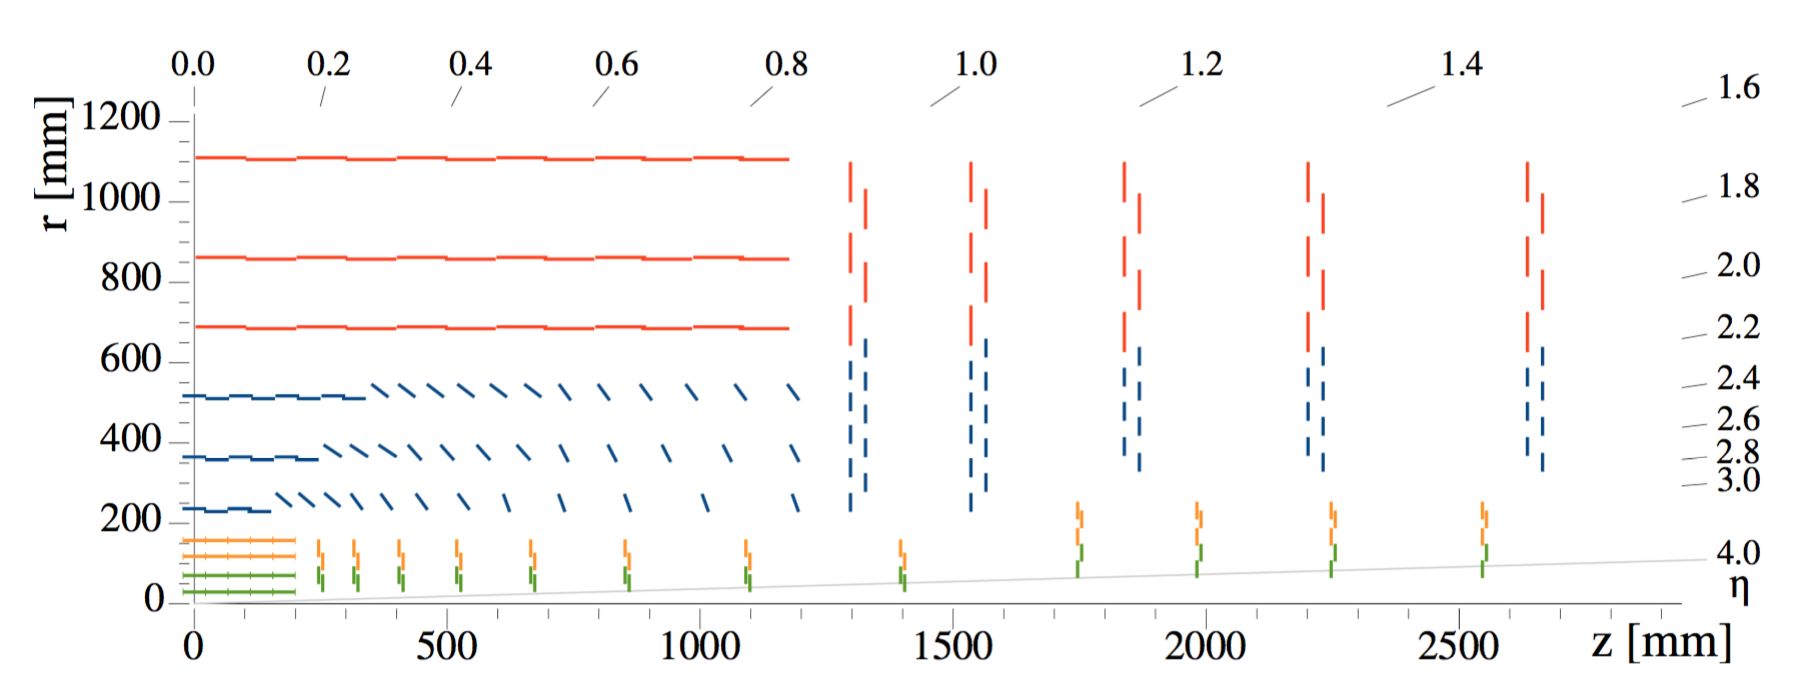
\includegraphics[width=0.9\textwidth]{Phase2TrackerLayout.png} 
\caption{ Sketch of one quarter of the tracker layout in r-z view. In the Inner Tracker the green lines correspond to pixel modules made of two readout chips and the yellow lines to pixel modules with four readout chips. In the Outer Tracker the blue and red lines represent the two types of modules  $p_\text{T}$ modules - (2S and PS).}
\label{Phase2TrackerLayout} 
\end{center}
\end{figure}

The OT will feature so-called ``$p_\text{T}$ modules'', which are capable of providing tracking information for the L1 trigger. The OT consists of six barrel layers (TBPS and TB2S) and five endcap double-discs (TEDD) which are composed of two types of $p_\text{T}$ modules, called 2S and PS modules. The first two endcap double-discs contain a total of 15 rings and the remaining three feature 12 rings each. This is shown in \autoref{OTlayout}.

\begin{figure}[H]
\begin{center}
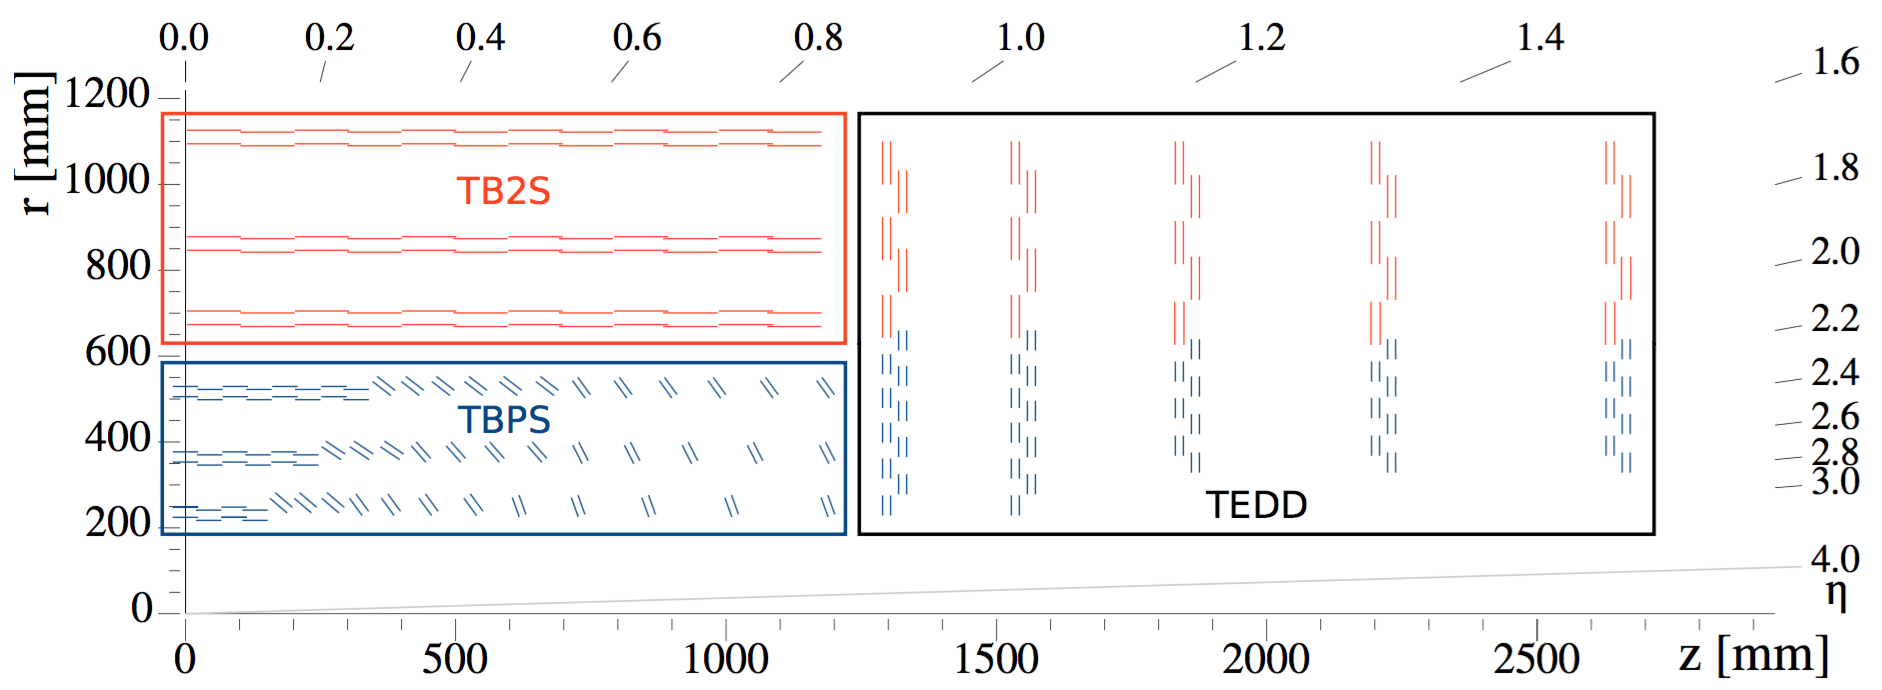
\includegraphics[width=0.9\textwidth]{OTlayout.png} 
\caption{Sketch of one quarter of the Outer Tracker in r-z view. Blue (red) lines represent PS (2S) modules. The three sub-detectors, named TBPS, TB2S, and TEDD, are indicated. All overlapping layers are shown separately.}
\label{OTlayout} 
\end{center}
\end{figure}

\begin{figure}[tb]
\begin{center}
\begin{minipage}[b]{0.45\textwidth}
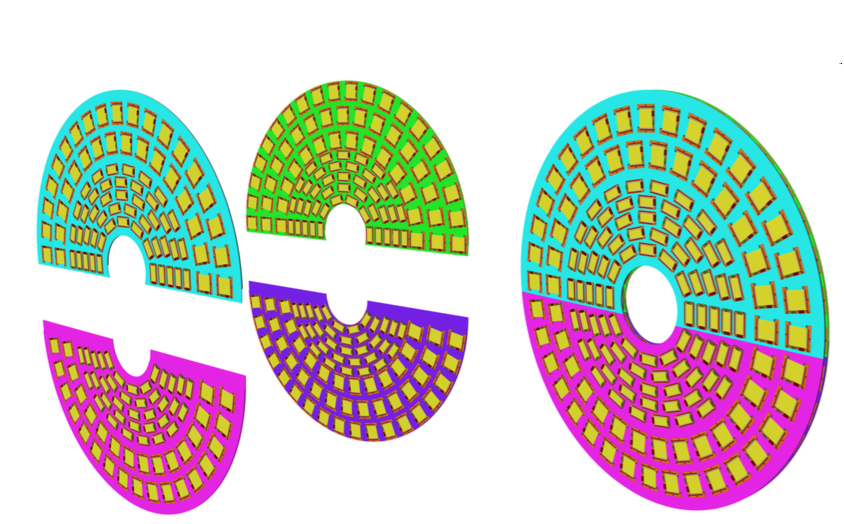
\includegraphics[width=\textwidth]{DoubleDisc.png} 
\end{minipage}
\hspace{1em}
\begin{minipage}[b]{0.45\textwidth}
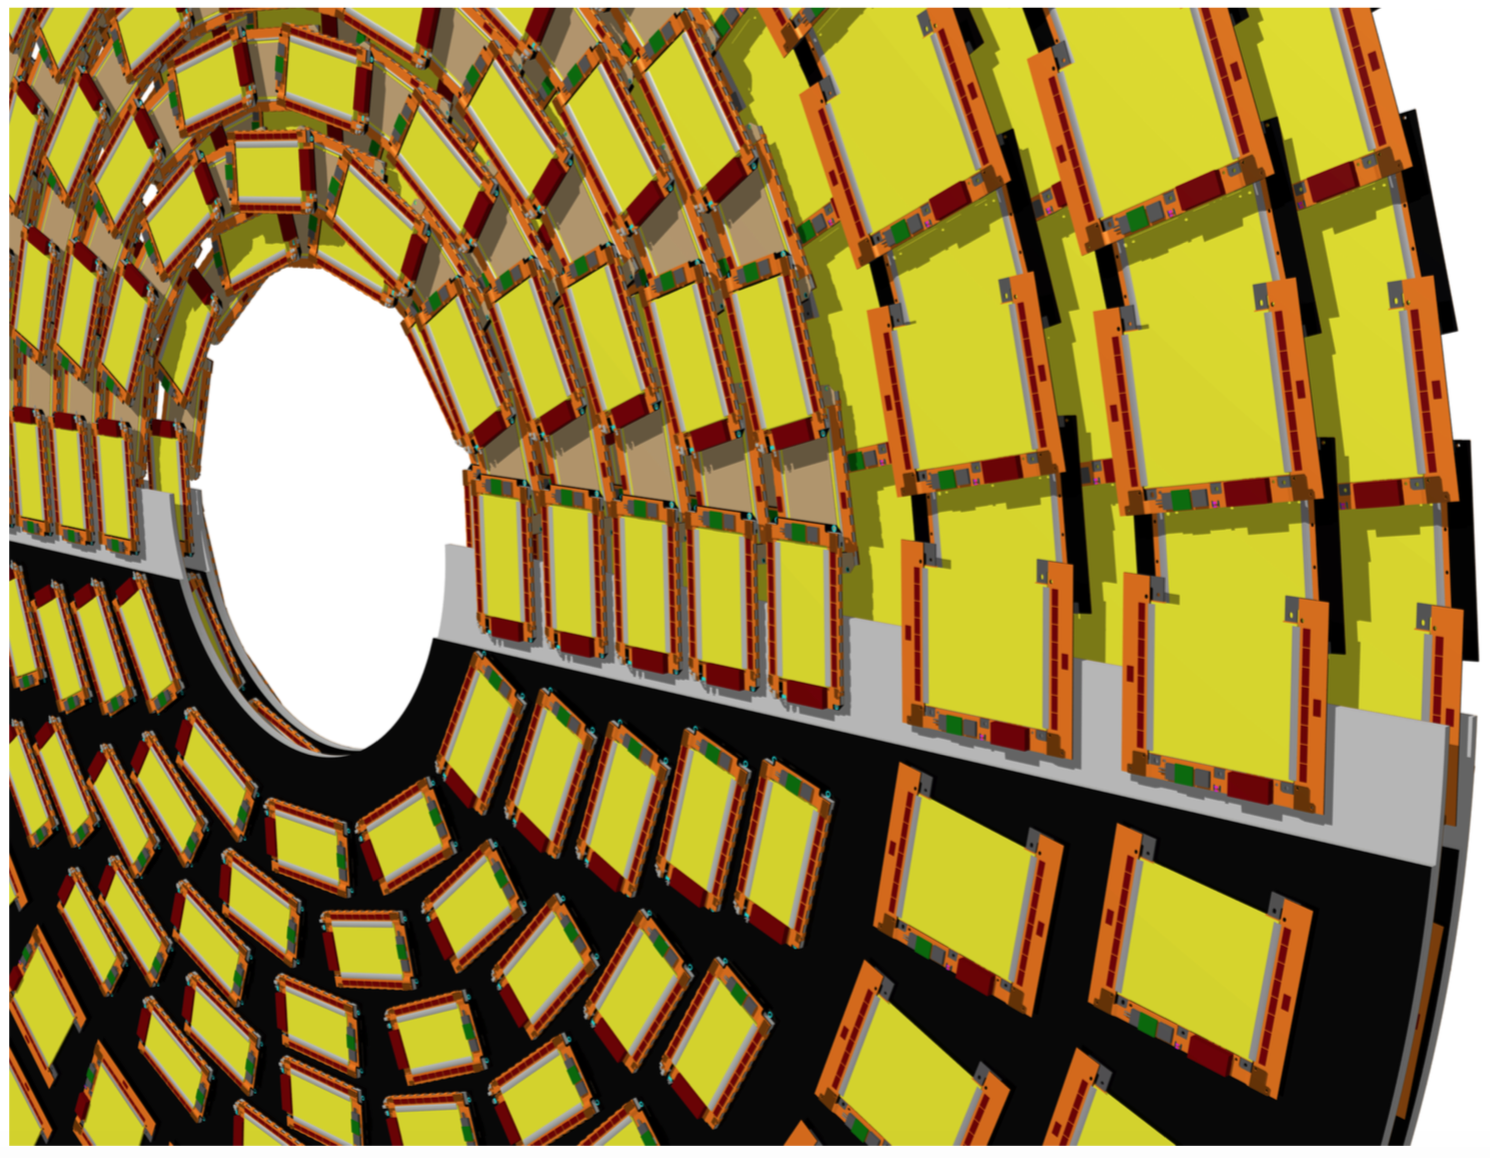
\includegraphics[width=\textwidth]{Phase2TEDD.png} 
\end{minipage}
\caption{Sketch of four dees (left) forming a double-disc (centre), and drawing of a part of a TEDD double-disc (right), illustrating the overlap of modules in $\phi$ and $z$. The upper two dee support structures are removed in order to show all layers of modules. The modules ob the disc are arranged in 15 or 12 rings.}
\label{Dees} 
\end{center}
\end{figure}

\subsection{Tracker Input to the L1-Trigger}\label{stubDefSec}

The enhancement of the trigger performance involves both a higher output rate of interesting events and an improved discriminating power of the event selection, which is more challenging in a high-pileup environment. Improved discriminating power will be achieved by using more information in the trigger decision, with a longer latency available for its processing. The use of tracking information in the L1 trigger will improve the $p_\text{T}$ resolution of various objects at L1 (e.g. jets), it will allow the exploitation of information on track isolation, and will contribute to the mitigation of pileup of 140-200 collisions per bunch crossing. CMS plans to enhance the first level trigger rate from presently 100 kHz to 750 kHz and to increase the latency from the present value of 3.2 $\mu s$ to 12.5 $\mu s$. The front-end electronics and the L1 trigger track reconstruction need to comply with these new requirements. The necessity of providing tracking information to the L1 trigger is a main driver for the design of the OT, including its module concept. The use of tracking information in the L1 trigger implies that the tracker has to send out self-selected information at every bunch crossing. Such functionality relies upon local data reduction in the front-end electronics, in order to limit the volume of data that has to be sent out at 40 MHz. This is achieved with modules that are capable of rejecting signals from particles below a certain $p_\text{T}$ threshold, referred to as ``$p_\text{T}$ modules'' \cite{Phase2Tracker1}. Tracks from charged particles are bent in the transverse plane by the 3.8 T field of the CMS magnet, with the bending angle depending on the $p_\text{T}$ of the particle. The modules are composed of two single-sided closely-spaced sensors read out by a common set of front-end ASICs that correlate the signals in the two sensors and select the hit pairs (referred to as ``stubs'') compatible with particles above the chosen $p_\text{T}$ threshold (as shown in \autoref{stubDef}). Stubs are defined as matching pairs of hits on the adjacent silicon layers of the $p_\text{T}$ modules. Whether or not a stub is accepted depends on the $p_\text{T}$ of the particle for a certain $p_\text{T}$ threshold value. 

\begin{figure}[tb]
\begin{center}
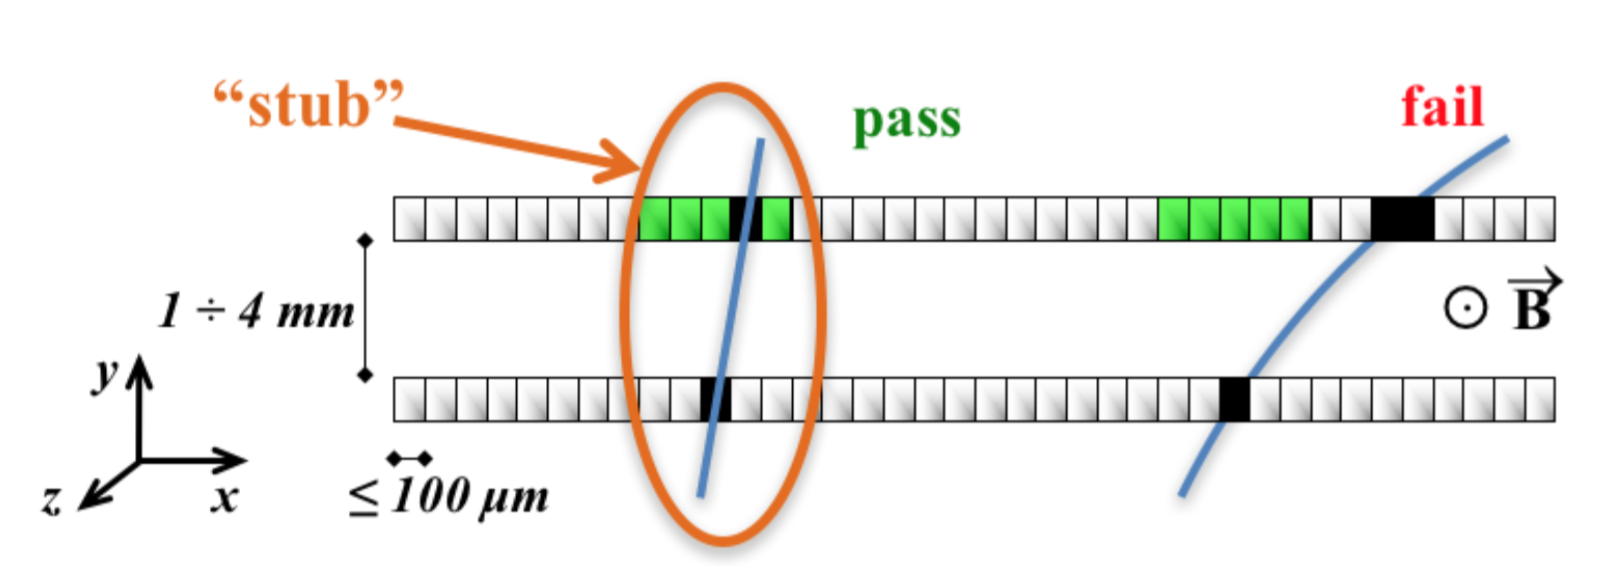
\includegraphics[width=0.9\textwidth]{stubDef.png} 
\caption{Correlation of signals in closely-spaced sensors enables rejection of low-$p_\text{T}$ particles; the channels shown in green represent the selection window to define an accepted stub.}
\label{stubDef} 
\end{center}
\end{figure}

\section{Tracker Stub Simulation}

The baseline detector design comprises a barrel part with 4 layers of TBPX, 8 small double-discs per side of TFPX and 4 large double-discs per side of TEPX. This forward and end part is referred to as $8l4s$ (8 TFPX and 4 TEPX). Any changes made to the detector design or its geometry, due to any circumstance, directly impacts the physics variables, such as tracking efficiency, fake rate, $p_\text{T}$ resolution, b-tagging and primary track reconstruction and needs to be simulated to understand its impact. The removal of discs from the Phase-2 Forward Pixel detector (TFPX/TEPX) would affect the production of L1 stubs in the upgraded CMS OT. A decrease in the total number of stubs is expected when less material is present due to secondary interactions.\\

To perform this study we considered the following four different geometries of the Pixel Detector:

\begin{itemize}
\item{8 small discs and 4 large discs ($8s4l$) -- designated as the default geometry}
\item{8 small discs and 3 large discs ($8s3l$) - one large disc removed.}
\item{7 small discs and 4 large discs ($7s4l$) -  one small disc removed.}
\item{6 small discs and 3 large discs ($6s3l$) - one large disc and two small discs removed.}
\item{A version of the default pixel geometry with a dead disc (used to verify our findings).}
\end{itemize}

\vspace{1em}

The response of the detector due to design modifications is simulated using the official CMS software package CMSSW. The detector geometry is generated with a design tool for innovative silicon tracking detectors called tkLayout \cite{tkLayout} and is exported into the standard CMSSW format along with the materials like sensing silicon elements, electronics and inactive material. The exported tracker geometry serves as input for the full simulation and reconstruction performance studies with CMSSW. The design of the CMS Phase-2 Tracker includes Tracker information for L1 triggering. The study was made from t$\bar{\text{t}}$ samples with a center-of-mass energy of 14 TeV and 200 pileup. The samples were created with the CMS software version referred to as CMSSW\_9\_3\_2. The stub information is used as input for the track fitting algorithm and allows tracks used for L1 trigger to be reconstructed within approximately 5 $\mu s$ (this includes a 1 $\mu s$ estimate for the time required to transmit the stub data from the detector to the counting room) to remain within the overall L1 trigger latency budget of 12.5 $\mu s$. Stubs are formed from two closely spaced sensors in Tracker measurement layers and provide linked position measurements for each particle passing through them. \autoref{SWtable} shows the stub window $p_\text{T}$ threshold values used for the study.

\begin{table}[tb]
\centering\footnotesize

\begin{tabular}{|c|c|ccc|l}
\cline{1-5}
\textbf{TEDD1} & \textbf{TEDD2} & \multicolumn{1}{c|}{\textbf{TEDD3}} & \multicolumn{1}{c|}{\textbf{TEDD4}} & \textbf{TEDD5} &  \\ \hline
5.5 & 5.5 & \multicolumn{1}{c|}{6.0} & \multicolumn{1}{c|}{6.5} & 6.5 & \multicolumn{1}{l|}{\textbf{R1}} \\ \hline
4.5 & 5.0 & \multicolumn{1}{c|}{5.5} & \multicolumn{1}{c|}{6.0} & 6.0 & \multicolumn{1}{l|}{\textbf{R2}} \\ \hline
3.5 & 4.0 & \multicolumn{1}{c|}{5.0} & \multicolumn{1}{c|}{6.0} & 6.0 & \multicolumn{1}{l|}{\textbf{R3}} \\ \hline
3.0 & 3.0 & \multicolumn{1}{c|}{2.5} & \multicolumn{1}{c|}{3.0} & 3.0 & \multicolumn{1}{l|}{\textbf{R4}} \\ \hline
2.5 & 2.0 & \multicolumn{1}{c|}{3.5} & \multicolumn{1}{c|}{3.0} & 3.0 & \multicolumn{1}{l|}{\textbf{R5}} \\ \hline
4.0 & 3.0 & \multicolumn{1}{c|}{2.5} & \multicolumn{1}{c|}{2.0} & 2.0 & \multicolumn{1}{l|}{\textbf{R6}} \\ \hline
3.5 & 3.0 & \multicolumn{1}{c|}{2.5} & \multicolumn{1}{c|}{2.0} & 2.0 & \multicolumn{1}{l|}{\textbf{R7}} \\ \hline
3.0 & 3.0 & \multicolumn{1}{c|}{2.5} & \multicolumn{1}{c|}{2.0} & 2.0 & \multicolumn{1}{l|}{\textbf{R8}} \\ \hline
3.0 & 2.5 & \multicolumn{1}{c|}{2.0} & \multicolumn{1}{c|}{2.0} & 1.5 & \multicolumn{1}{l|}{\textbf{R9}} \\ \hline
2.5 & 2.0 & \multicolumn{1}{c|}{2.0} & \multicolumn{1}{c|}{1.5} & 1.5 & \multicolumn{1}{l|}{\textbf{R10}} \\ \hline
2.0 & 2.0 & \multicolumn{1}{c|}{1.5} & \multicolumn{1}{c|}{1.5} & 1.5 & \multicolumn{1}{l|}{\textbf{R11}} \\ \hline
2.0 & 2.0 & \multicolumn{1}{c|}{1.5} & \multicolumn{1}{c|}{1.0} & 1.0 & \multicolumn{1}{l|}{\textbf{R12}} \\ \hline
1.5 & 1.5 &  &  &  & \multicolumn{1}{l|}{\textbf{R13}} \\ \cline{1-2} \cline{6-6} 
1.5 & 1.5 &  &  &  & \multicolumn{1}{l|}{\textbf{R14}} \\ \cline{1-2} \cline{6-6} 
1.0 & 1.0 &  &  &  & \multicolumn{1}{l|}{\textbf{R15}} \\ \cline{1-2} \cline{6-6} 
\end{tabular}

\vspace{1em}

\centering\scriptsize
\resizebox{\textwidth}{!}{%
\begin{tabular}{l|c|c|c|c|c|c|c|c|c|c|c|c|c|}
\hline
\multicolumn{1}{|l|}{\textbf{TB2S3}} & \multicolumn{13}{c|}{6.5} \\ \hline
\multicolumn{1}{|l|}{\textbf{TB2S2}} & \multicolumn{13}{c|}{5.5} \\ \hline
\multicolumn{1}{|l|}{\textbf{TB2S1}} & \multicolumn{13}{c|}{4.5} \\ \hline
\multicolumn{1}{|l|}{\textbf{TBPS3}} & 3.5 & 4.5 & 4.5 & 4.0 & 4.0 & 4.0 & 4.0 & 3.5 & 3.5 & 3.5 & 3.0 & 3.0 & 3.0 \\ \hline
\multicolumn{1}{|l|}{\textbf{TBPS2}} & 2.0 & 3.0 & 3.0 & 3.0 & 3.0 & 2.5 & 2.5 & 2.5 & 2.5 & 2.5 & 2.5 & 2.0 & 2.0 \\ \hline
\multicolumn{1}{|l|}{\textbf{TBPS1}} & 2.0 & 2.5 & 2.5 & 2.5 & 2.5 & 2.5 & 2.5 & 2.0 & 2.0 & 1.5 & 1.5 & 1.0 & 1.0 \\ \hline
 & \textbf{FLAT} & \textbf{R1} & \textbf{R2} & \textbf{R3} & \textbf{R4} & \textbf{R5} & \textbf{R6} & \textbf{R7} & \textbf{R8} & \textbf{R9} & \textbf{R10} & \textbf{R11} & \textbf{R12} \\ \cline{2-14} 
\end{tabular}%
}
\caption{Stub window tunings for CMSSW\_9\_3\_2. Shown are the SW values for TEDD (top table) and for the OT barrel (below). Obtained from \href{https://github.com/cms-sw/cmssw/blob/CMSSW\_9\_3\_X/L1Trigger/TrackTrigger/python/TTStubAlgorithmRegister\_cfi.py} {this github repository}.}
\label{SWtable}
\end{table}

\vspace{1em}

\begin{figure}[H]
\begin{center}
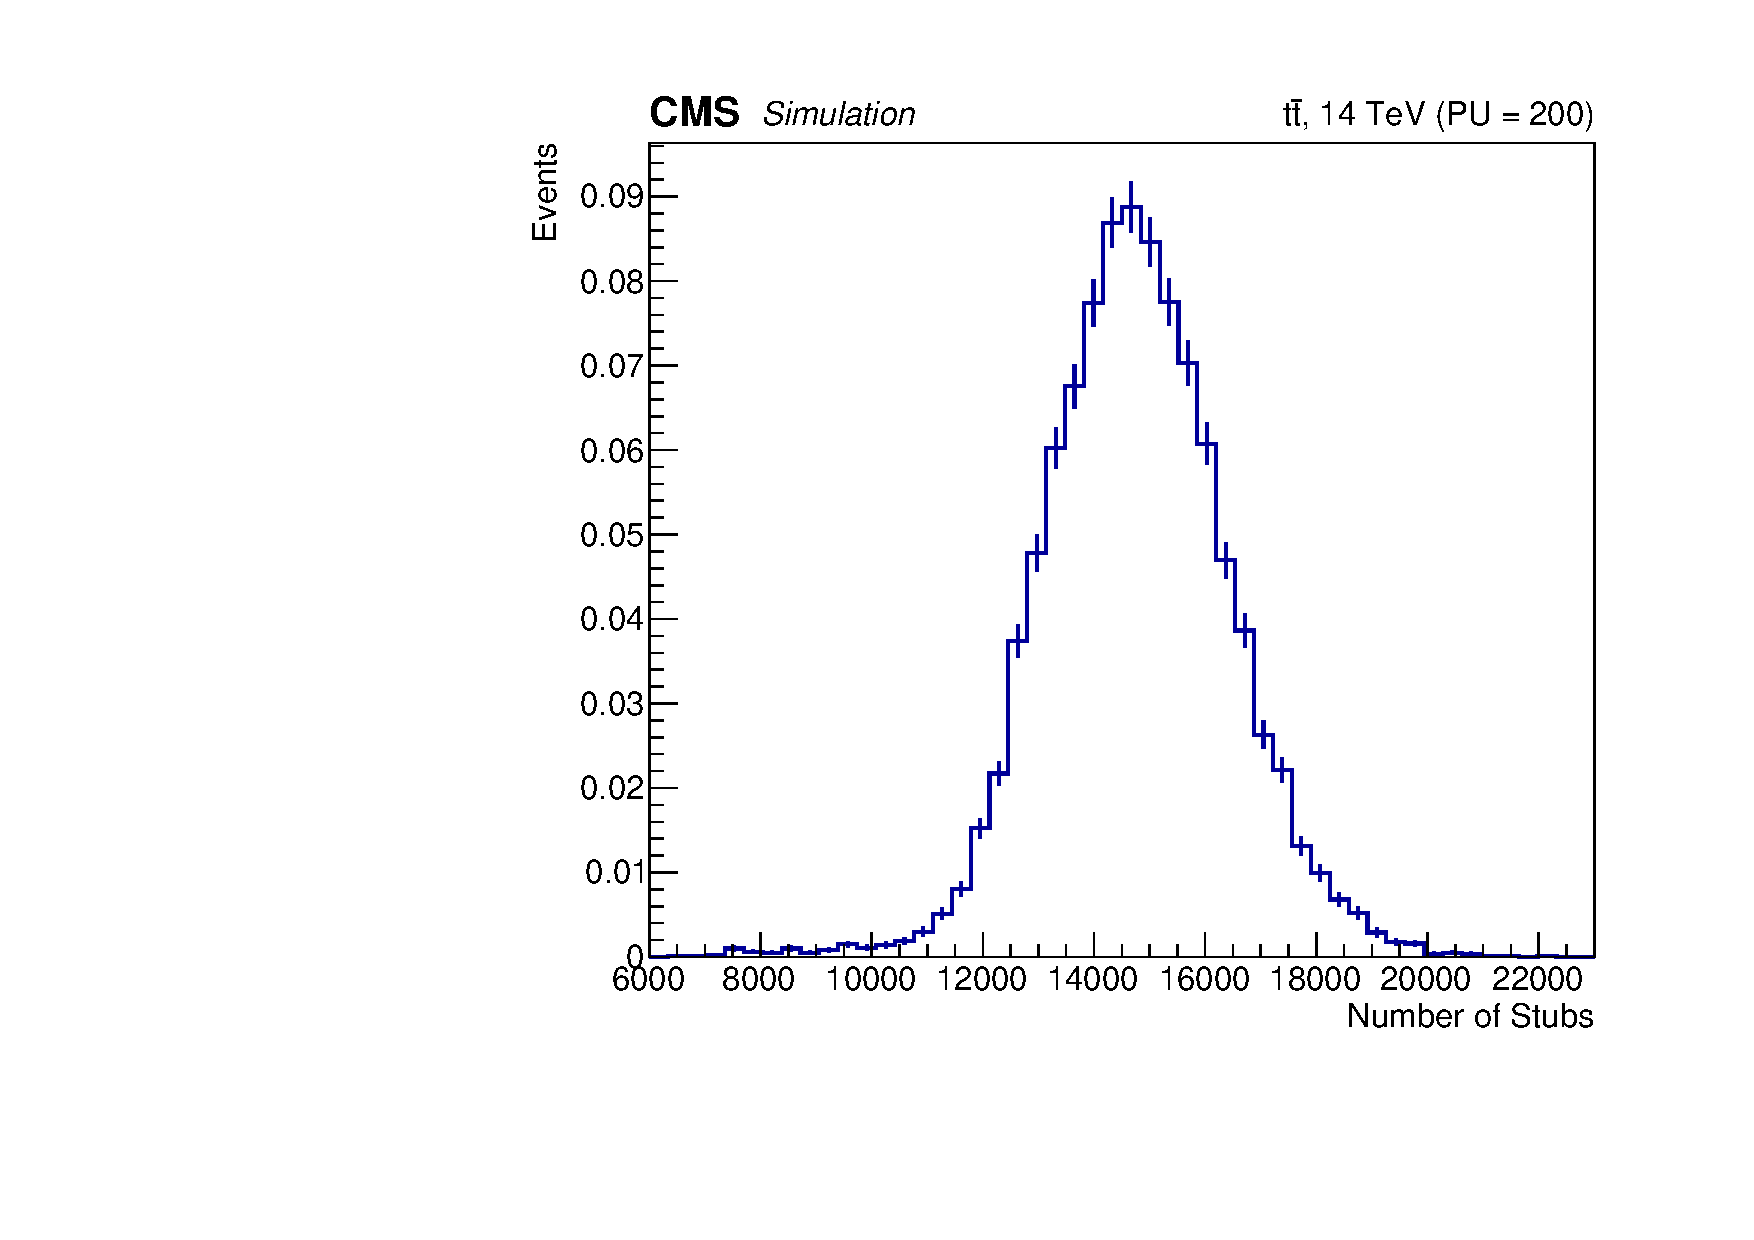
\includegraphics[width=0.65\textwidth]{nstub_8s4l_Single.pdf} 
\caption{Number of stubs per event for standard pixel geometry ($8s4l$).}
\label{nstub8s4l} 
\end{center}
\end{figure}

\subsection{Results of Effect of the Phase 2 Pixel Detector on the L1 Stub Rate}

\begin{enumerate}[(a),start=1]
	\item{\textbf{Number of Stubs:} With the current (above table) stub window tuning, the total number of stubs are on average $\sim$15,000 stubs as shown in \autoref{nstub8s4l}.}
\end{enumerate}

\begin{figure}[H]
    \centering
    \subfigure{
    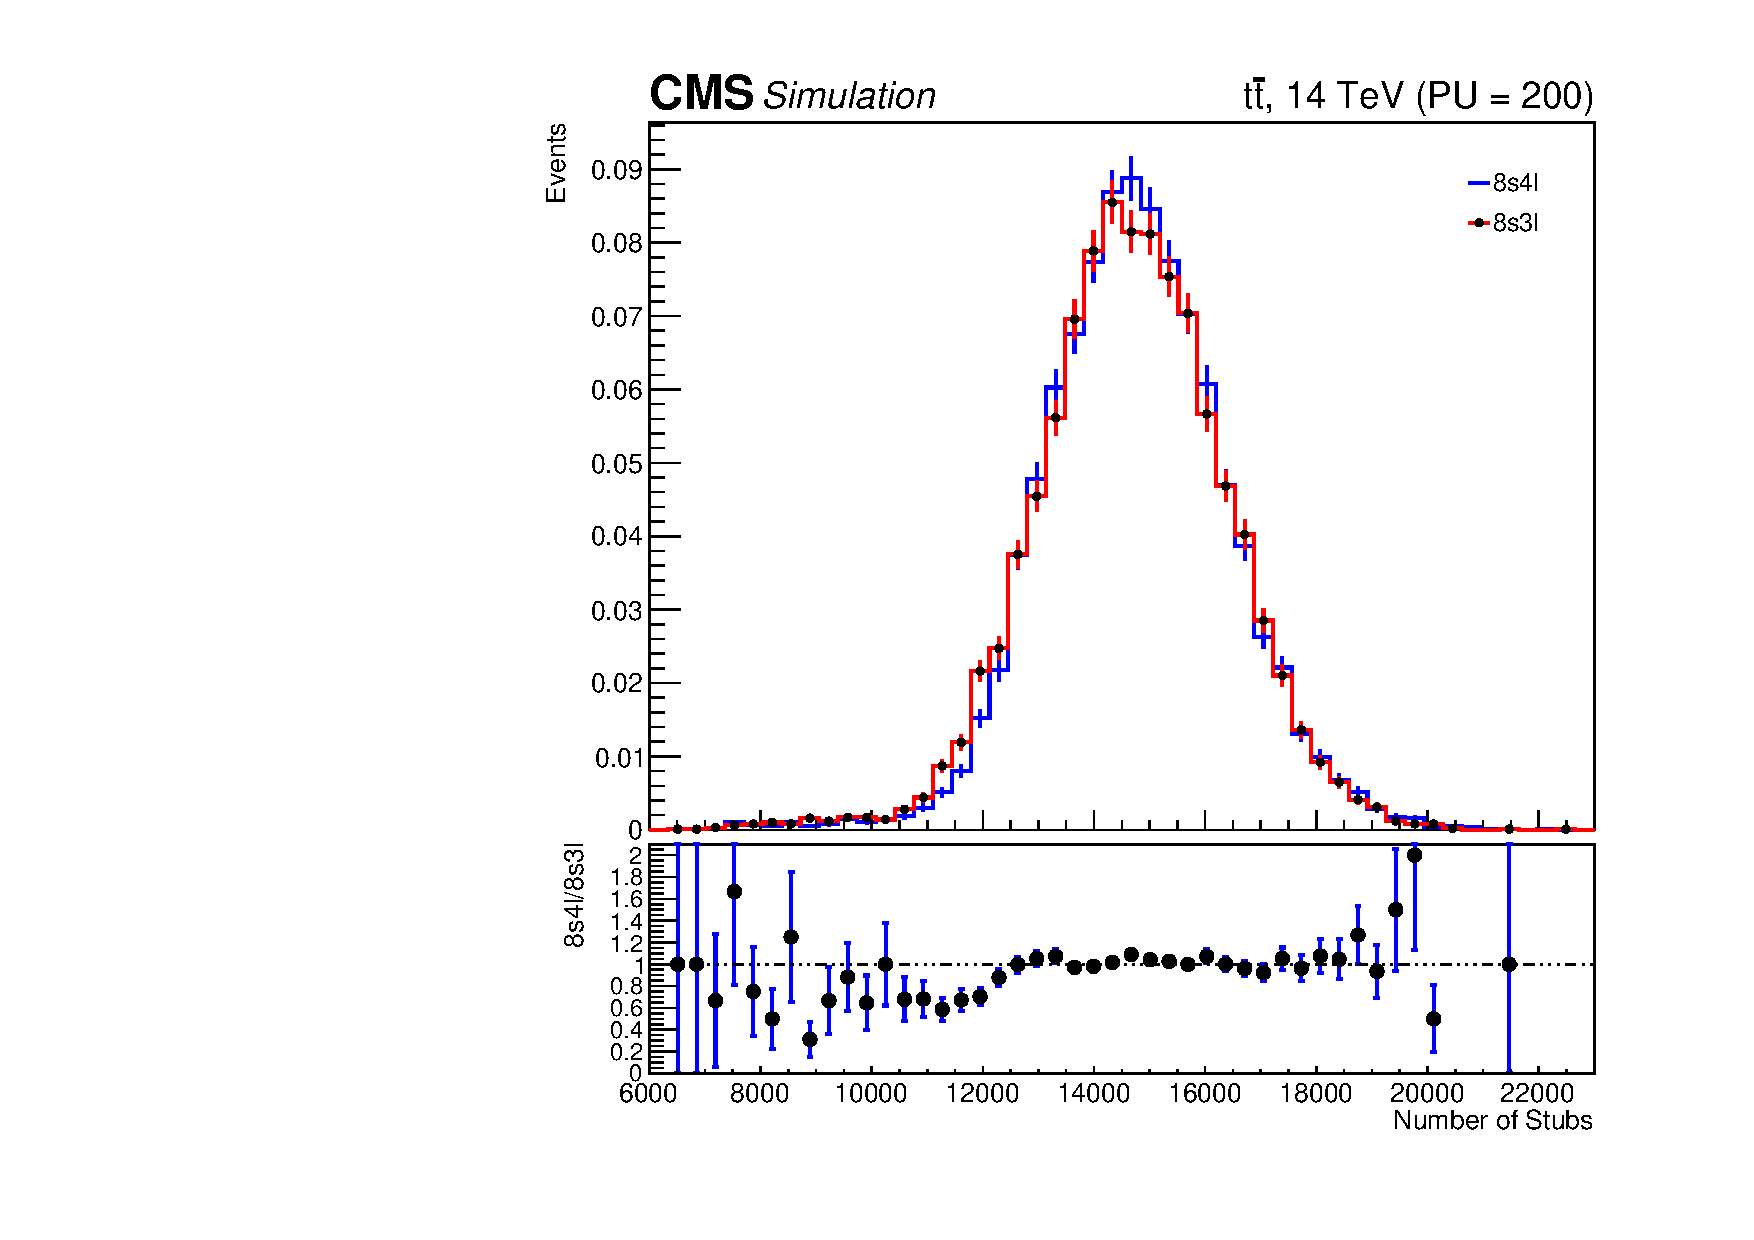
\includegraphics[width=0.32\textwidth]{nstub_8s4l_vs_8s3l_ratio.pdf}}
     \subfigure{
     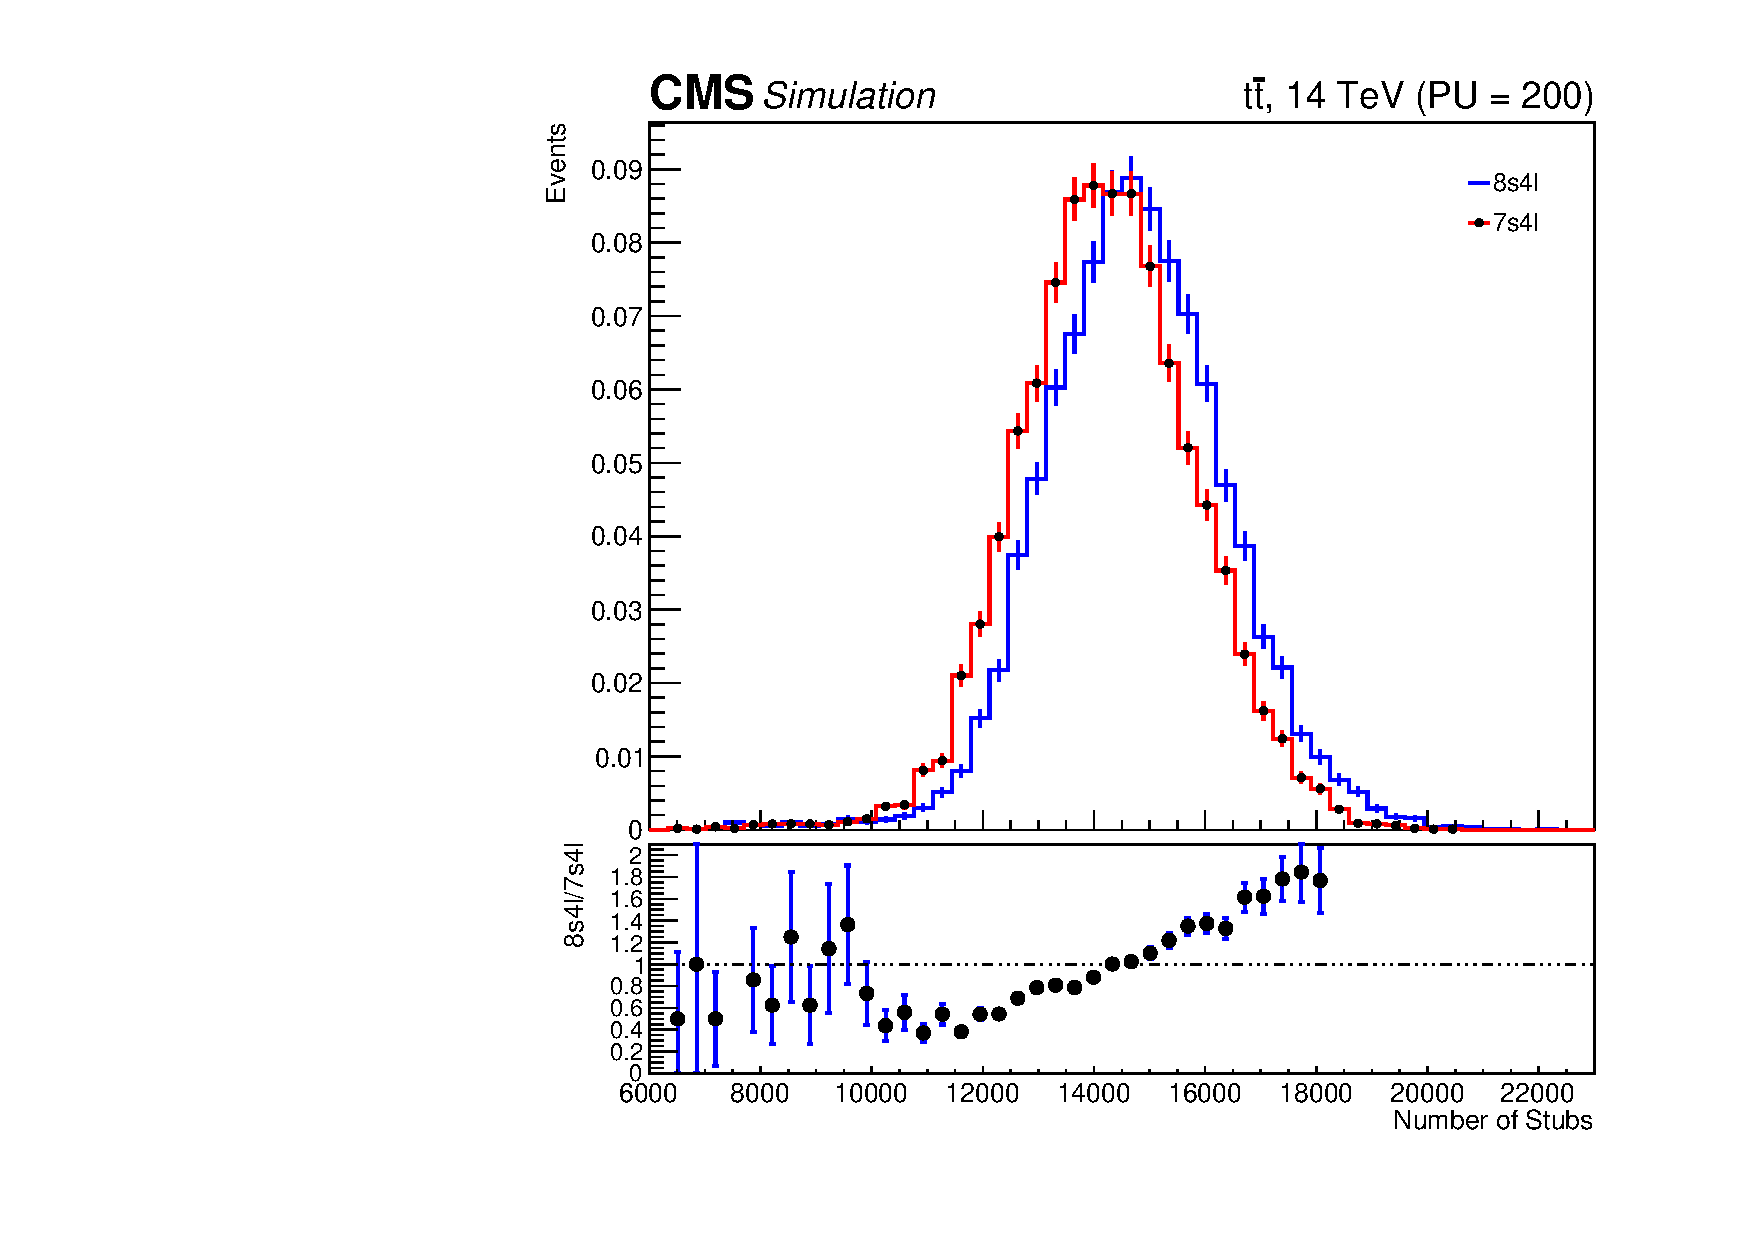
\includegraphics[width=0.32\textwidth]{nstub_8s4l_vs_7s4l_ratio.pdf}}
     \subfigure{
     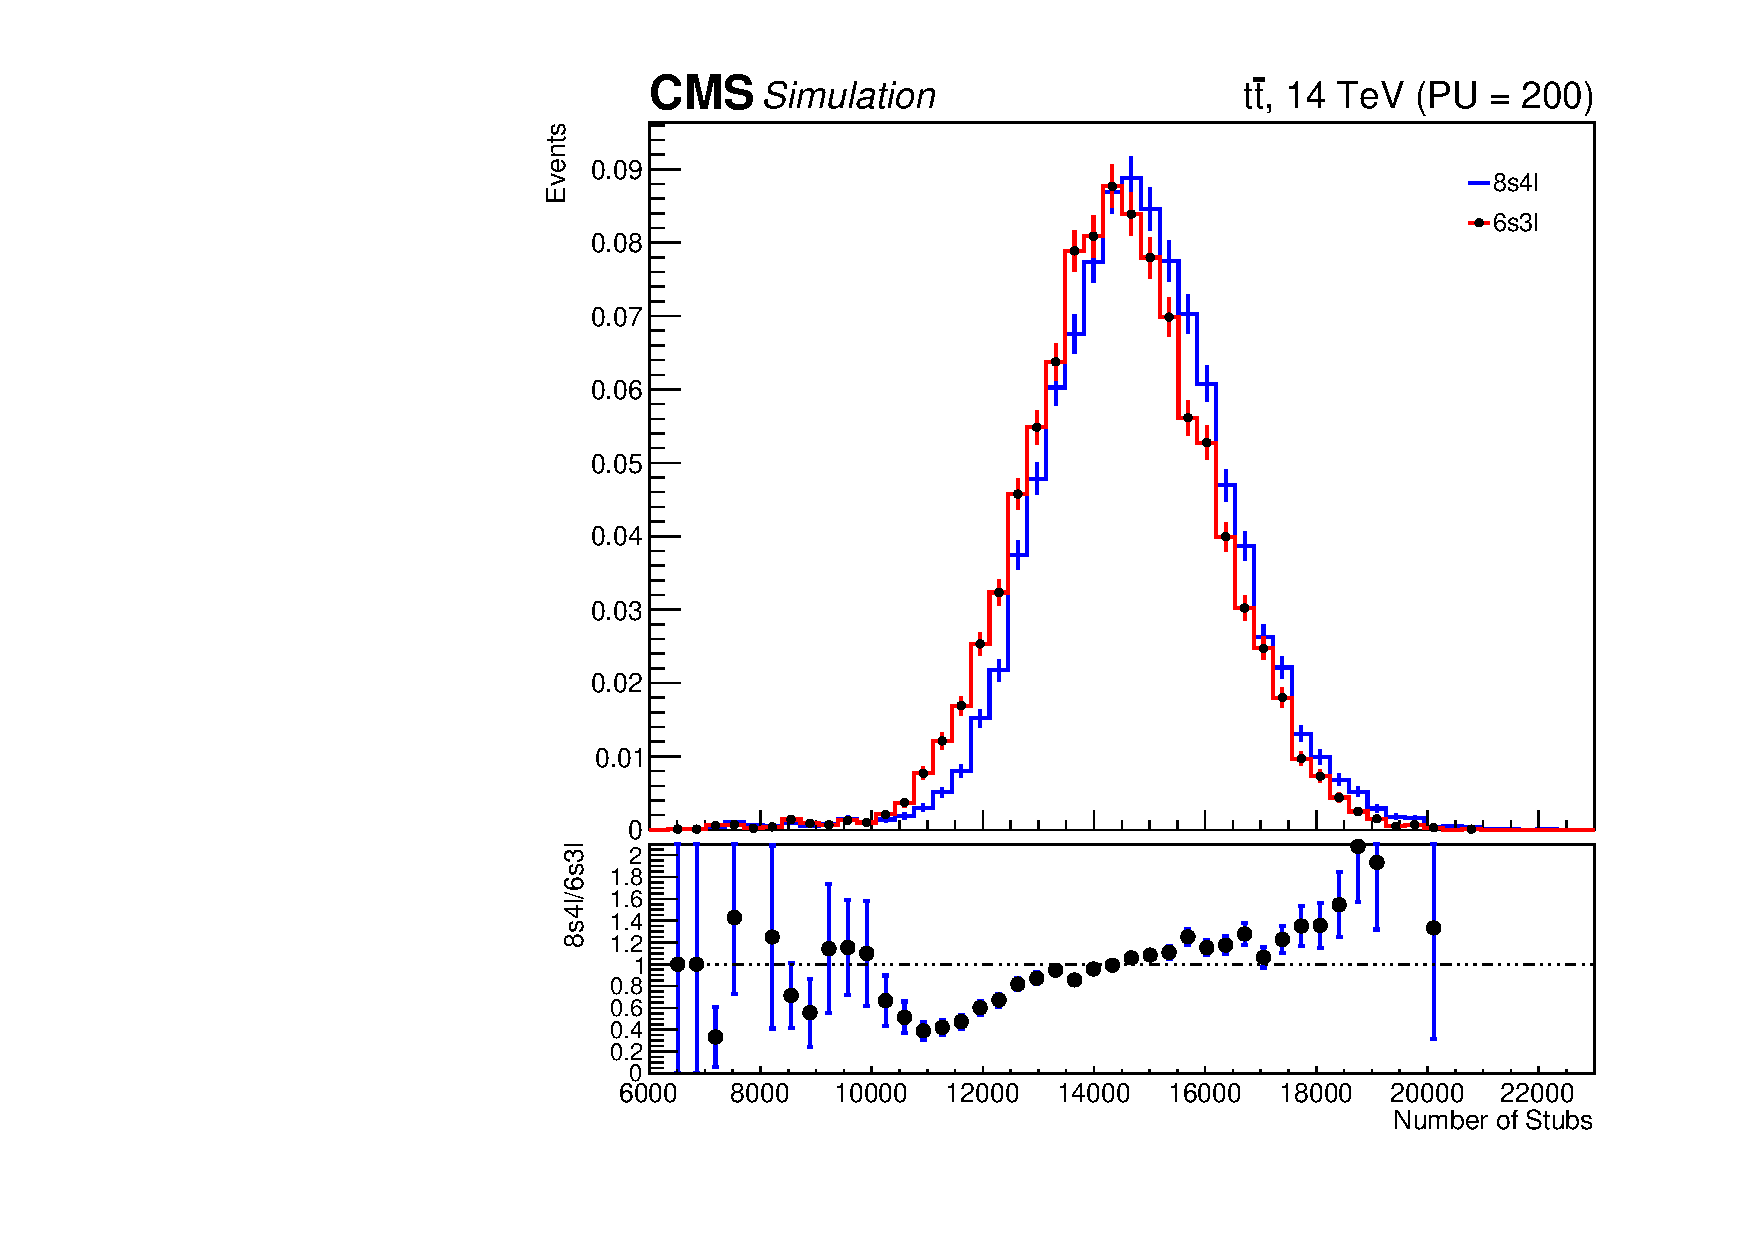
\includegraphics[width=0.32\textwidth]{nstub_8s4l_vs_6s3l_ratio.pdf}}
     \caption{Comparison of total number of stubs per event between the standard layout and the other three considered. $8s4l$ vs $8s3l$ (left), $8s4l$ vs $7s4l$ (middle) and $8s4l$ vs $6s3l$ (right).}
\label{nstubComp}
\end{figure}

\vspace{1em}

\begin{enumerate}[(a),resume]	
	\item{\textbf{Comparison of Stubs between default Pixel Geometry (8s4l) to disc removed:}}
\end{enumerate}

A comparison of the total number of stubs per event between the standard geometry to the others that have a disc or more removed ($8s3l$, $7s4l$, $6s3l$) was performed (\autoref{nstubComp}). Out of the three comparisons shown, the largest shift in the stub distribution can be seen from the $7s4l$ geometry. It was found that the removal of a smaller pixel disc has a more pronounced effect on stub production in the OT than a larger pixel disc.\\

\begin{figure}[H]
\begin{center}
\begin{minipage}[b]{0.45\textwidth}
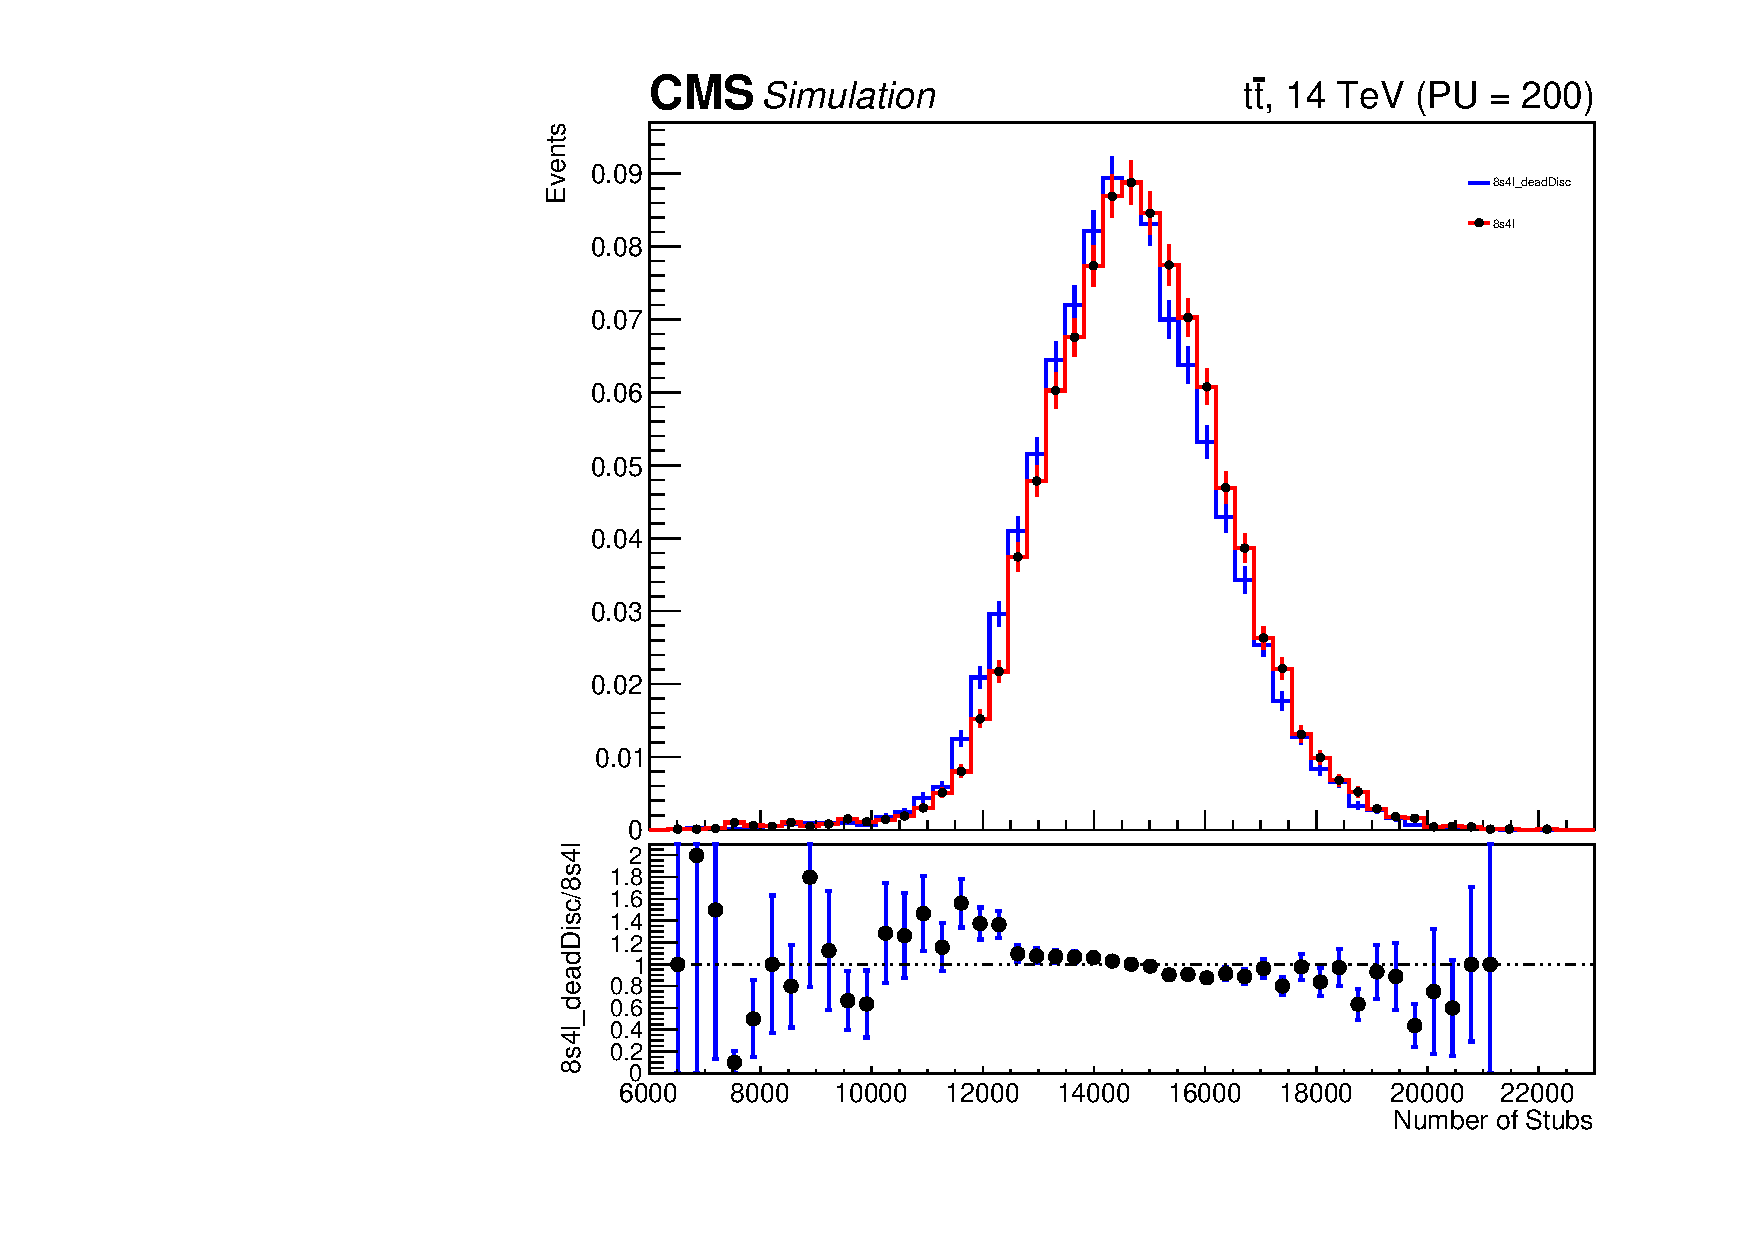
\includegraphics[width=\textwidth]{nstub_8s4l_deadDisc_vs_8s4l_ratio.pdf} 
\end{minipage}
\hspace{1em}
\begin{minipage}[b]{0.45\textwidth}
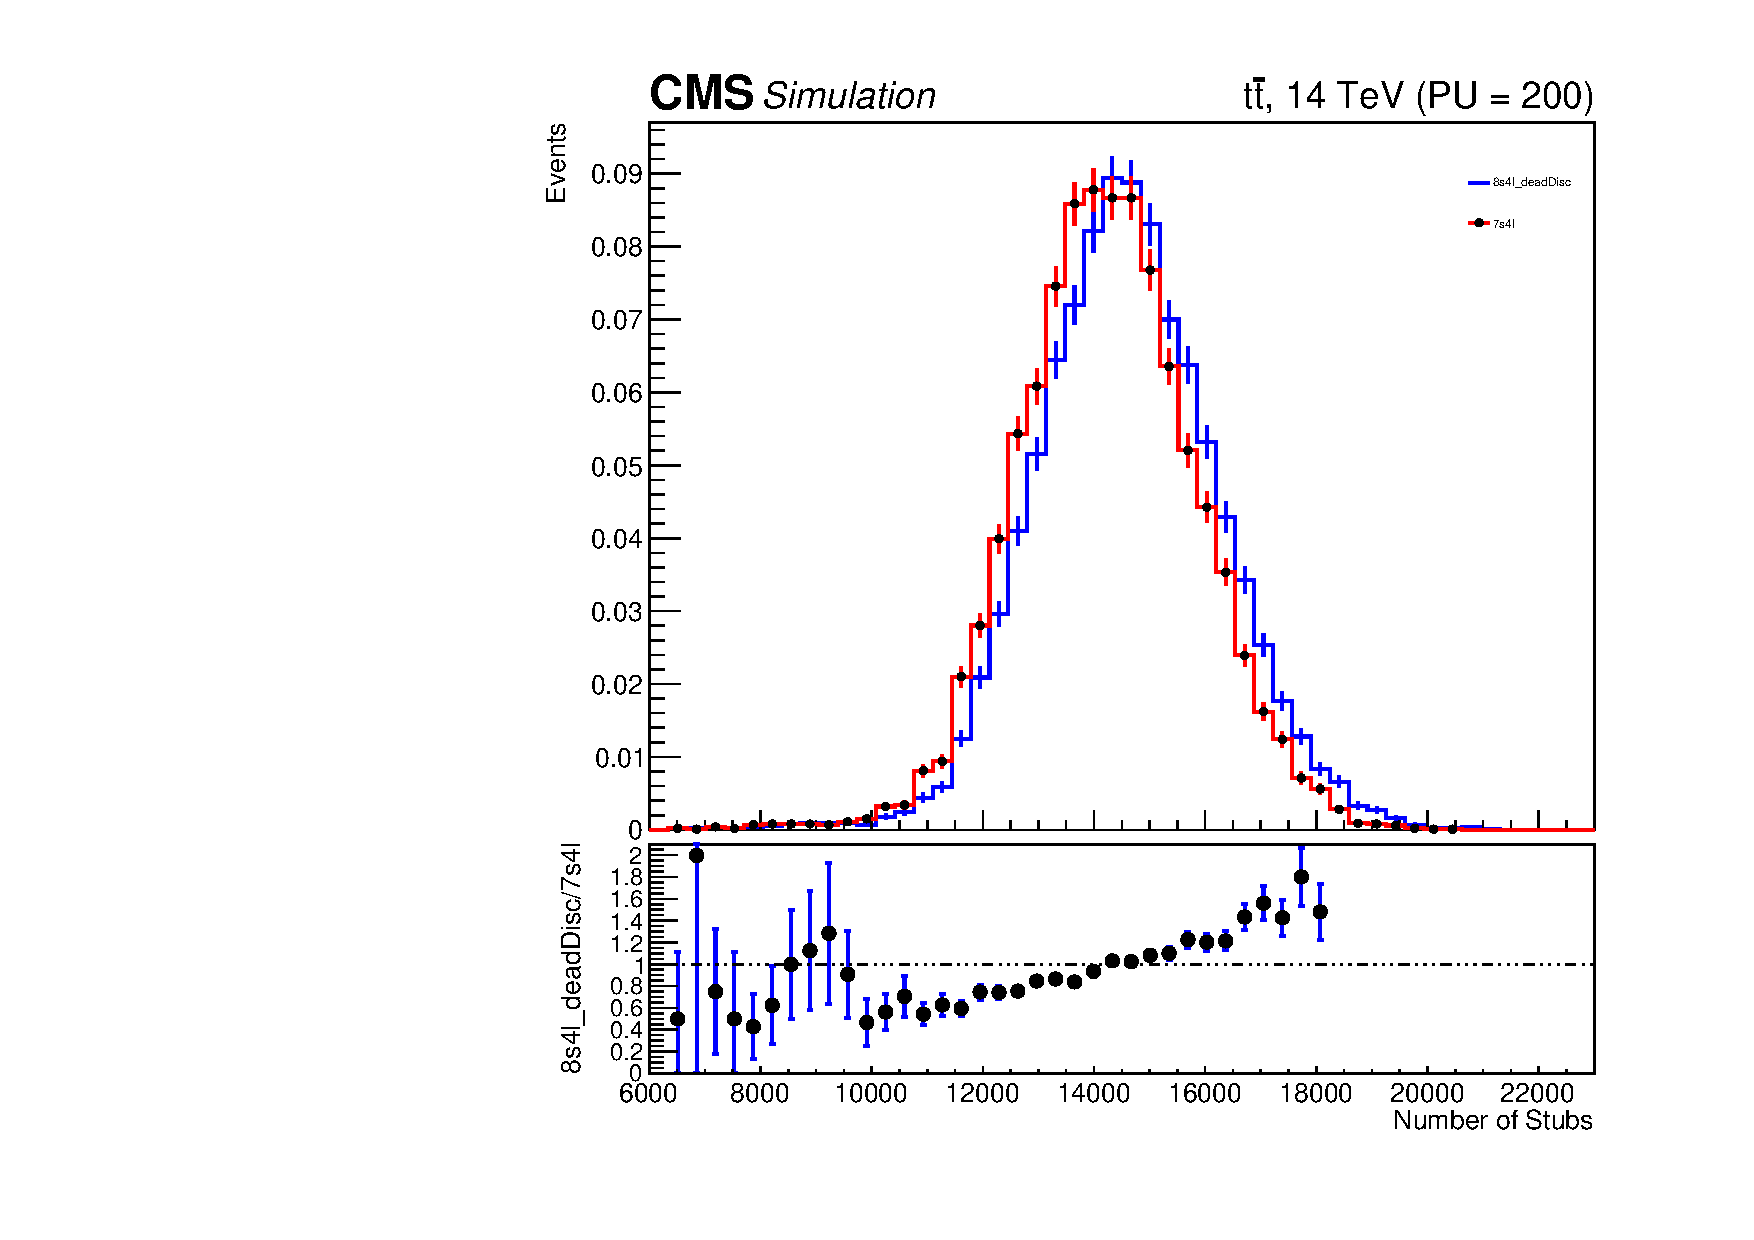
\includegraphics[width=\textwidth]{nstub_8s4l_deadDisc_vs_7s4l_ratio.pdf} 
\end{minipage}
\caption{Comparison for number of stubs per event between pixel geometry 8s4l with a dead disc (blue) and both pixel geometry $8s4l$ (right plot) and $7s4l$ (left plot) (blue). Both the standard geometry and $7s4l$ are shown in blue in their respective plots.}
\label{nstubdeadDisc} 
\end{center}
\end{figure}

\begin{enumerate}[(a),resume]
\item{\textbf{Comparison with a disc dead in default geometry:}}
\end{enumerate}

An additional study, using pixel geometry $8s4l$ with a dead disc, was made to verify the effect observed on the L1 stub counting.\autoref{nstubdeadDisc} (right) shows a comparison between 2 geometries that are (in principle) identical but one detects no hits on the second disc in the positive side. This Figure shows a slight deviation from the original $8s4l$ geometry.\\

Comparing the number of stubs for the geometry with the dead disc (blue) to the one with the removed small disc (red), the same behavior (\autoref{nstubdeadDisc}, left) is observed as before. As was expected, the stub distribution for pixel geometry $8s4l$ has a higher mean value than $7s4l$, despite the dead disc. The removal of discs in the pixel detector causes the total number of stubs to decrease due to secondary interactions with the material. We also studied the effect of the pixel geometries on the stubs with respect to the pseudorapidity ($\eta$) as shown in \autoref{stubEtaComp}. 

\begin{figure}[H]
    \centering
    \subfigure{
    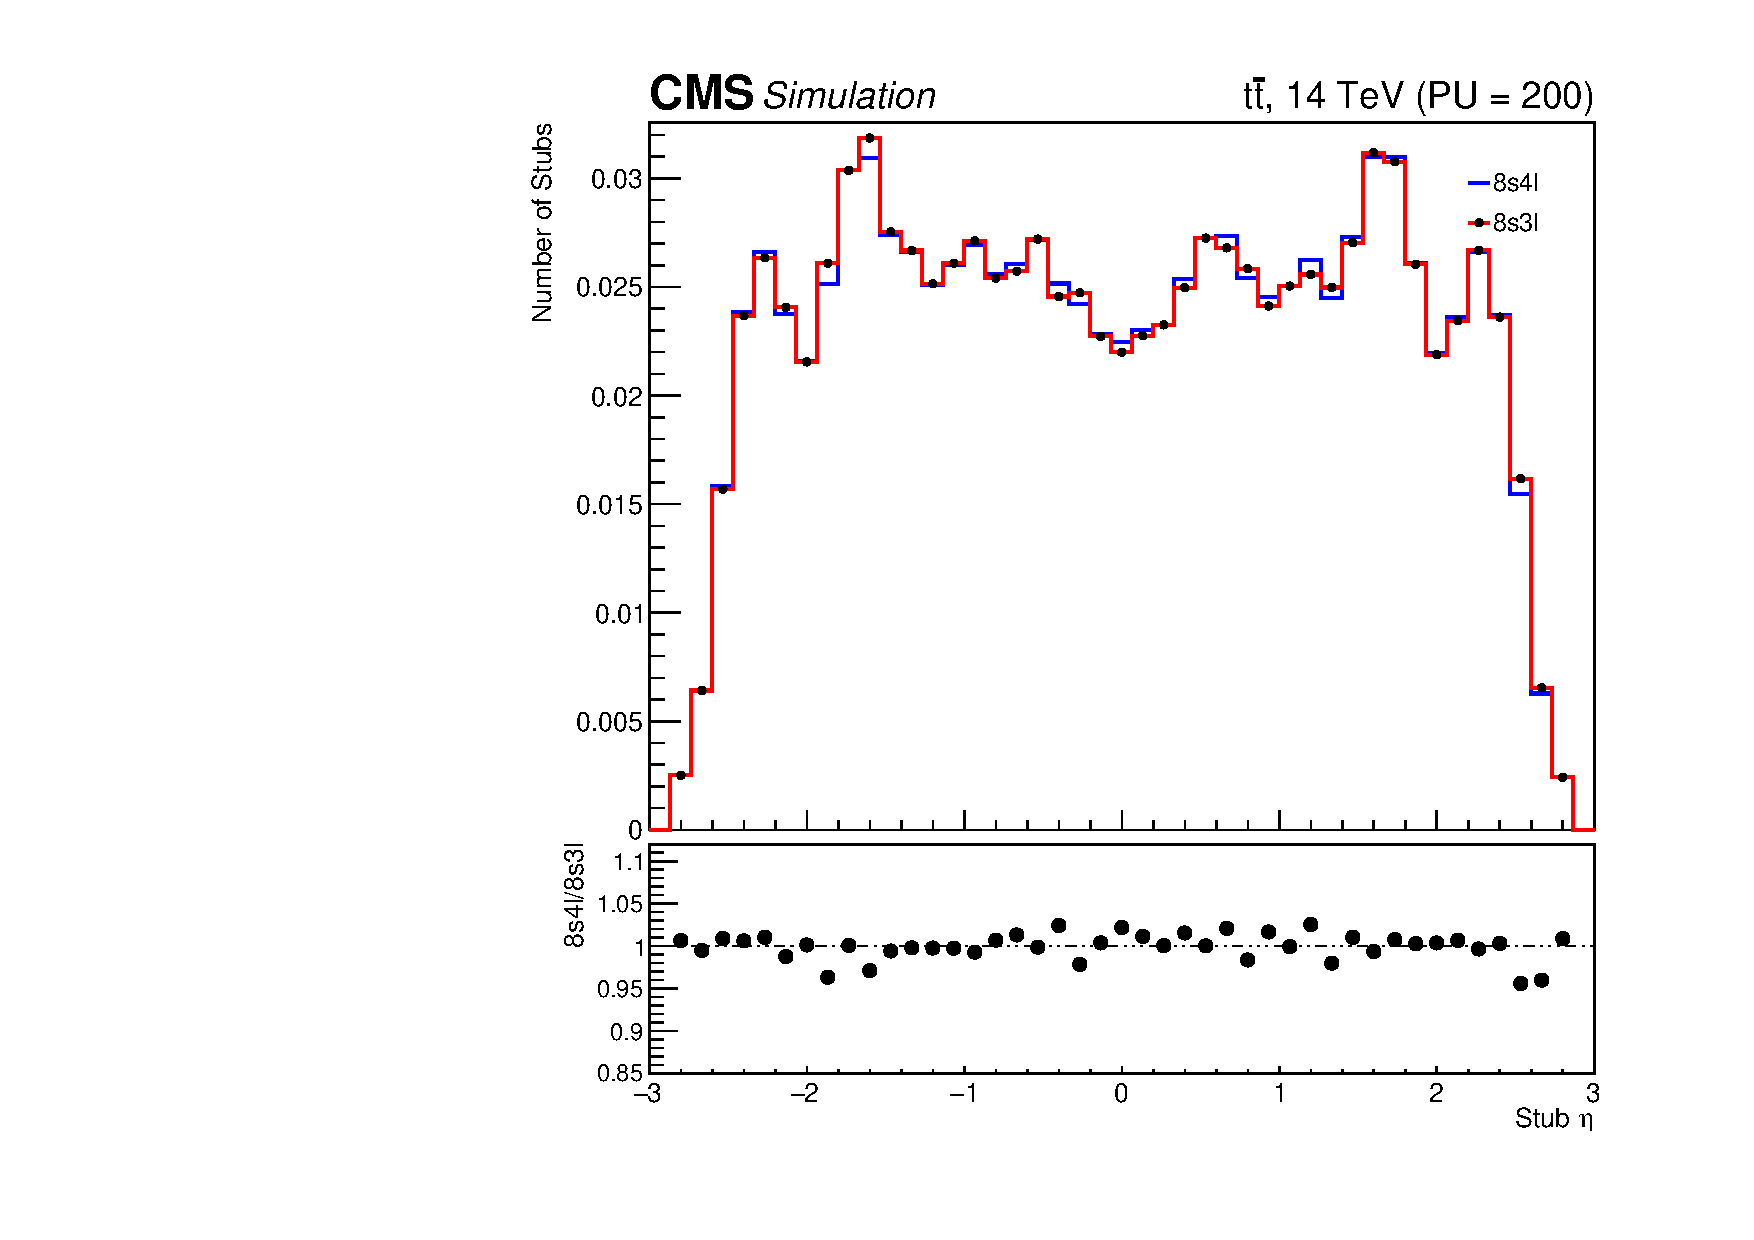
\includegraphics[width=0.32\textwidth]{Stub_Eta_8s4l_vs_8s3l_ratio.pdf}}
     \subfigure{
     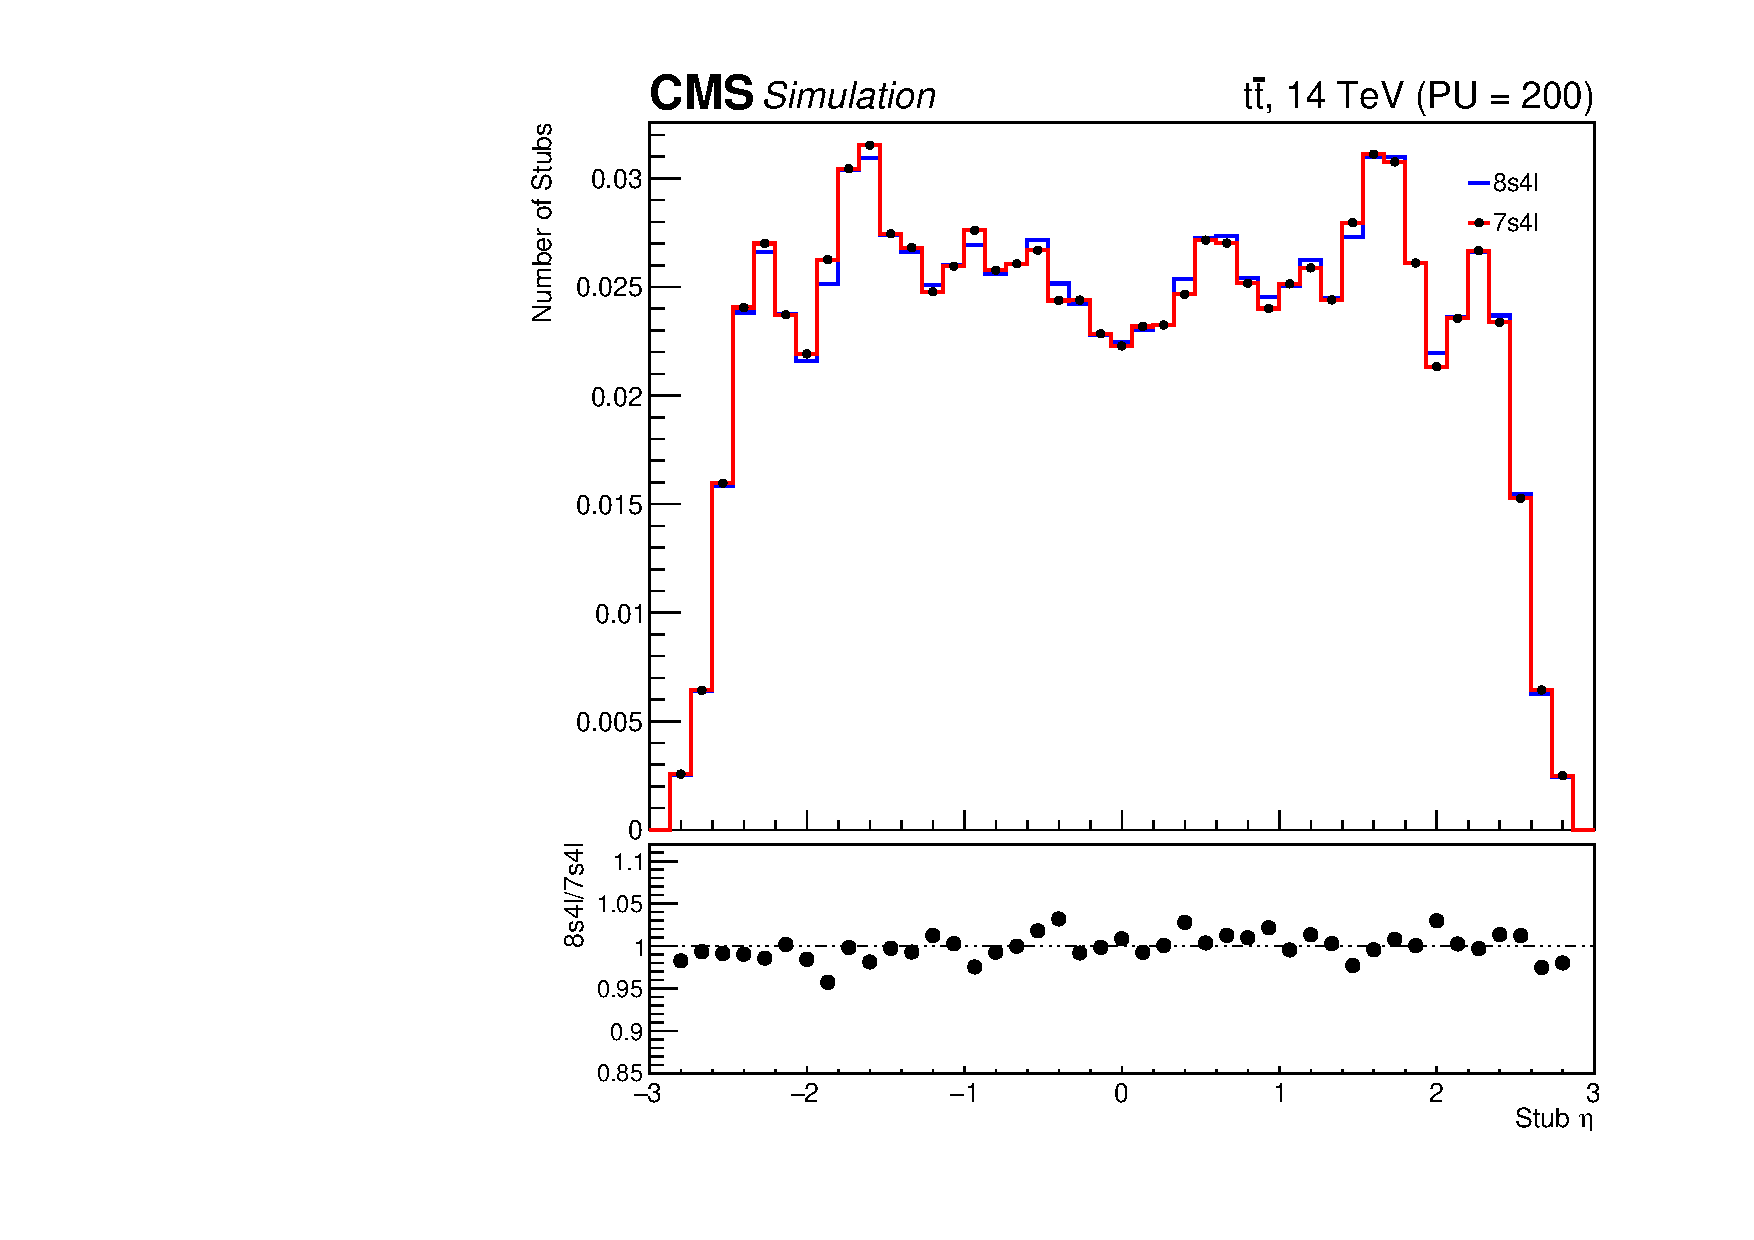
\includegraphics[width=0.32\textwidth]{Stub_Eta_8s4l_vs_7s4l_ratio.pdf}}
     \subfigure{
     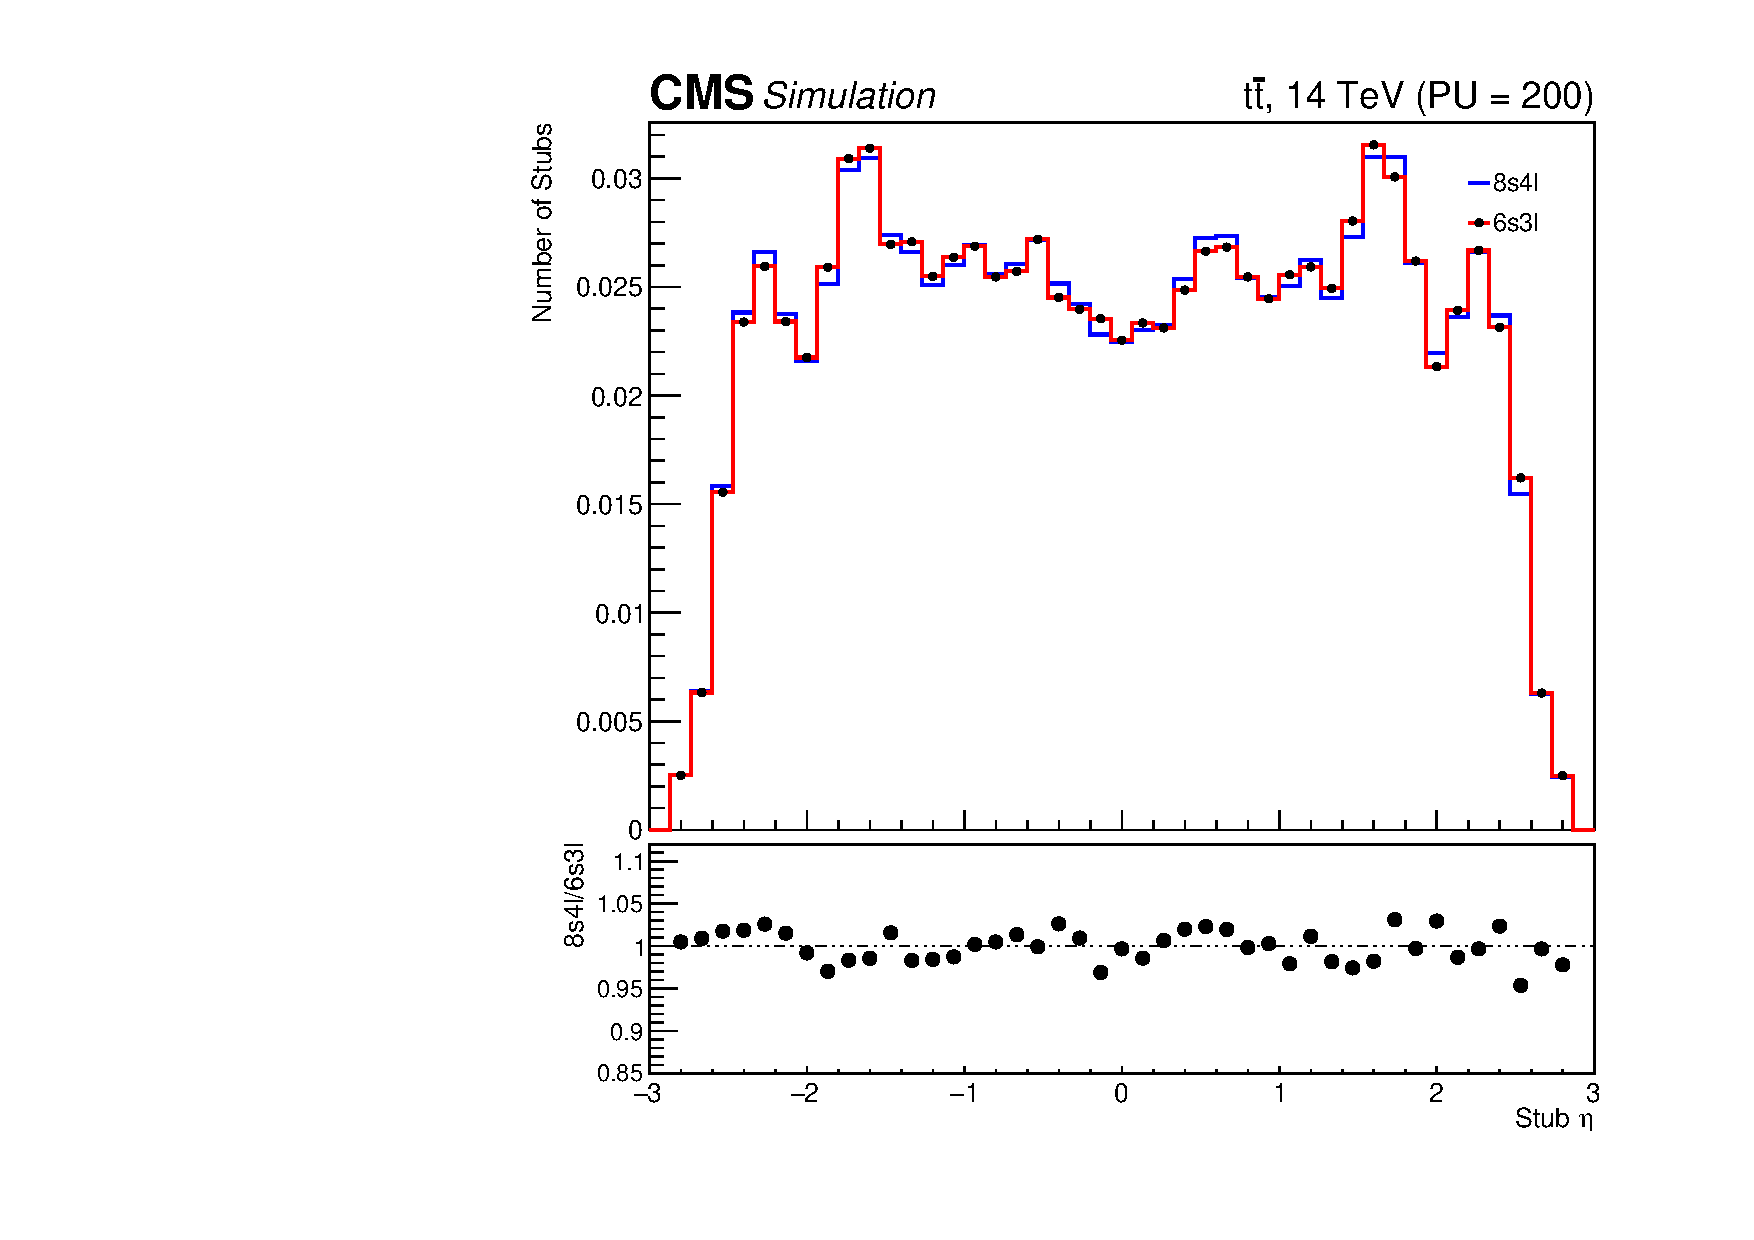
\includegraphics[width=0.32\textwidth]{Stub_Eta_8s4l_vs_6s3l_ratio.pdf}}
     \caption{Comparison of total number of stubs per $\eta$ value between the standard layout and the other three layouts considered. All four different layouts exhibit the same distribution. $8s4l$ vs $8s3l$ (left), $8s4l$ vs $7s4l$ (middle) and $8s4l$ vs $6s3l$ (right).}
\label{stubEtaComp}
\end{figure}

\vspace{1em}

We further studied the effect of the pixel geometries on the stubs per barrel (\autoref{stubsBarrel}), end discs (\autoref{stubsEndcap}) of the OT and per ring of the endcap discs (\autoref{stubsPerRing}).

\begin{figure}[H]
    \centering
    \subfigure{
    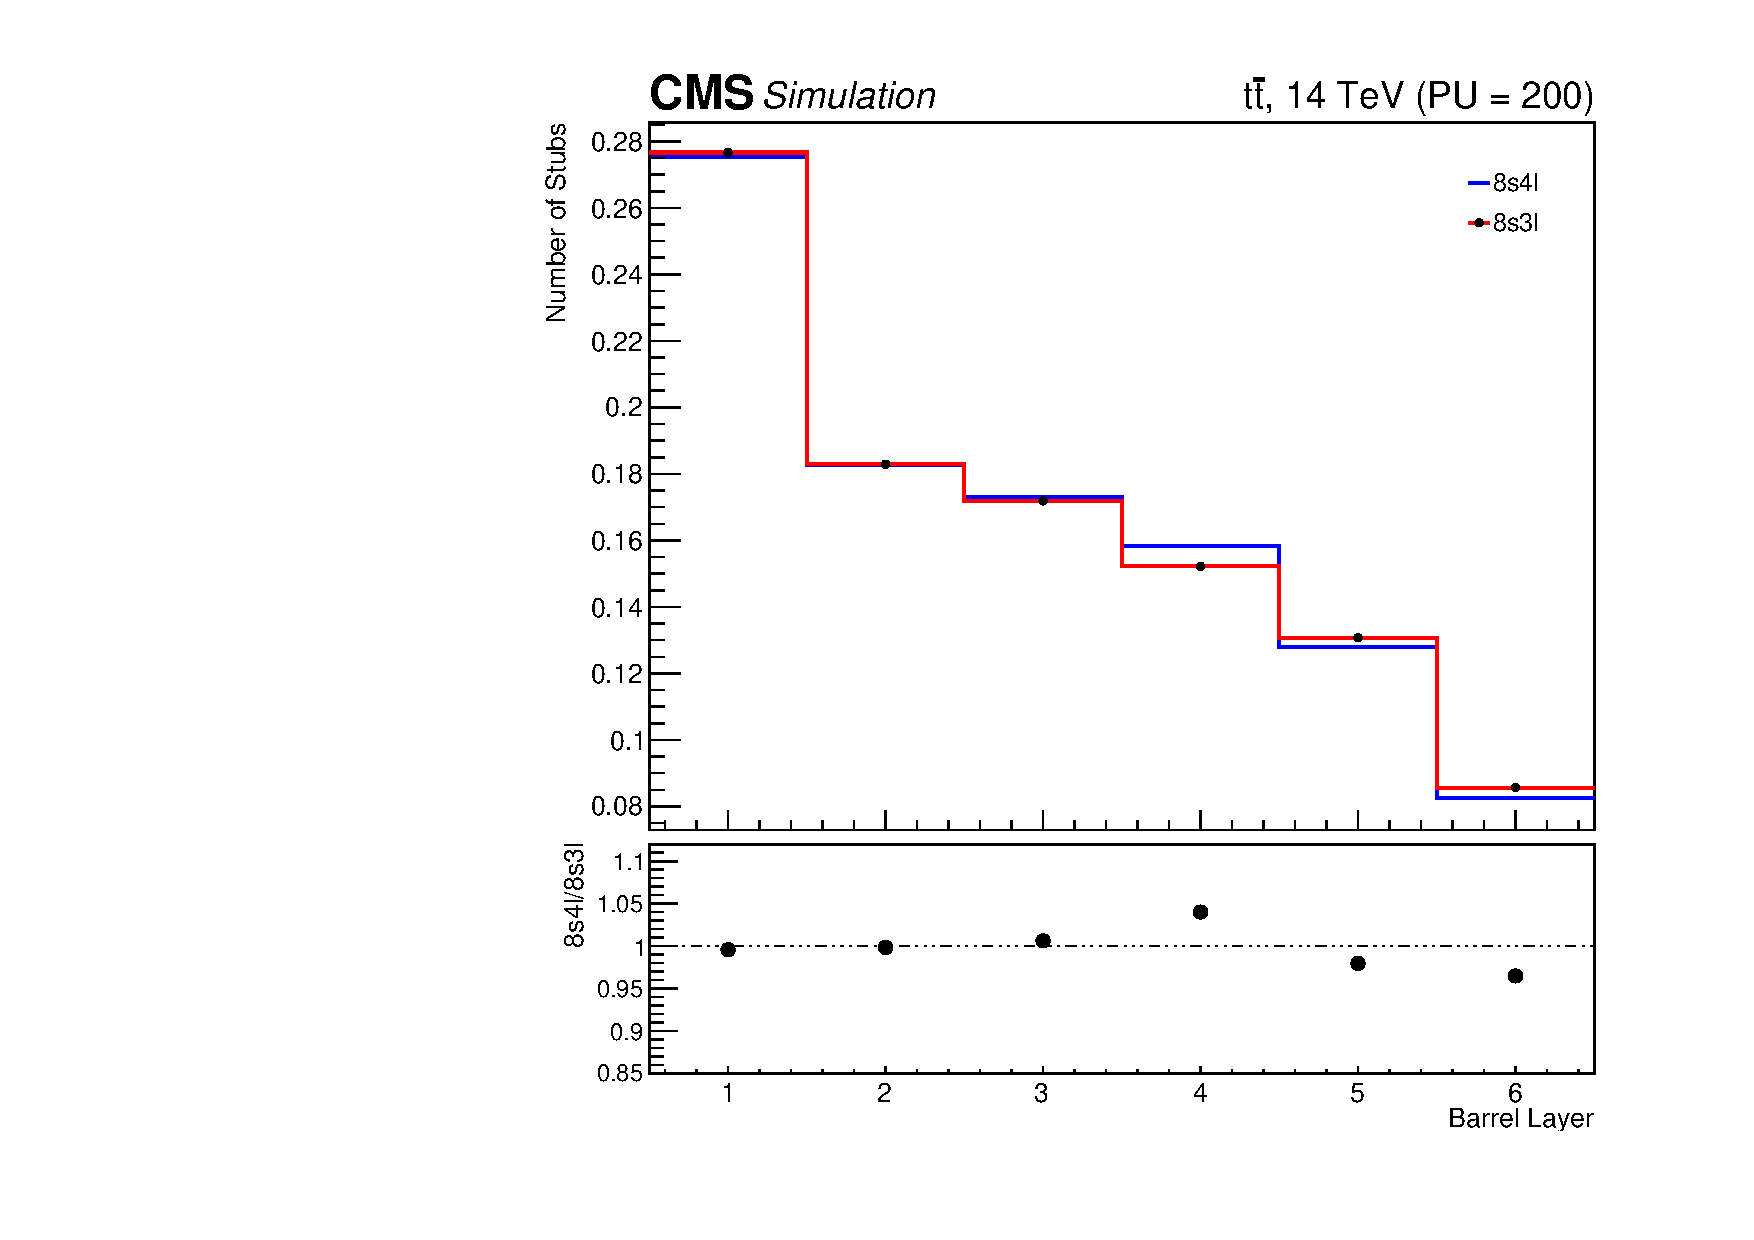
\includegraphics[width=0.32\textwidth]{NStubs_Barrel_8s4l_vs_8s3l_ratio.pdf}}
     \subfigure{
     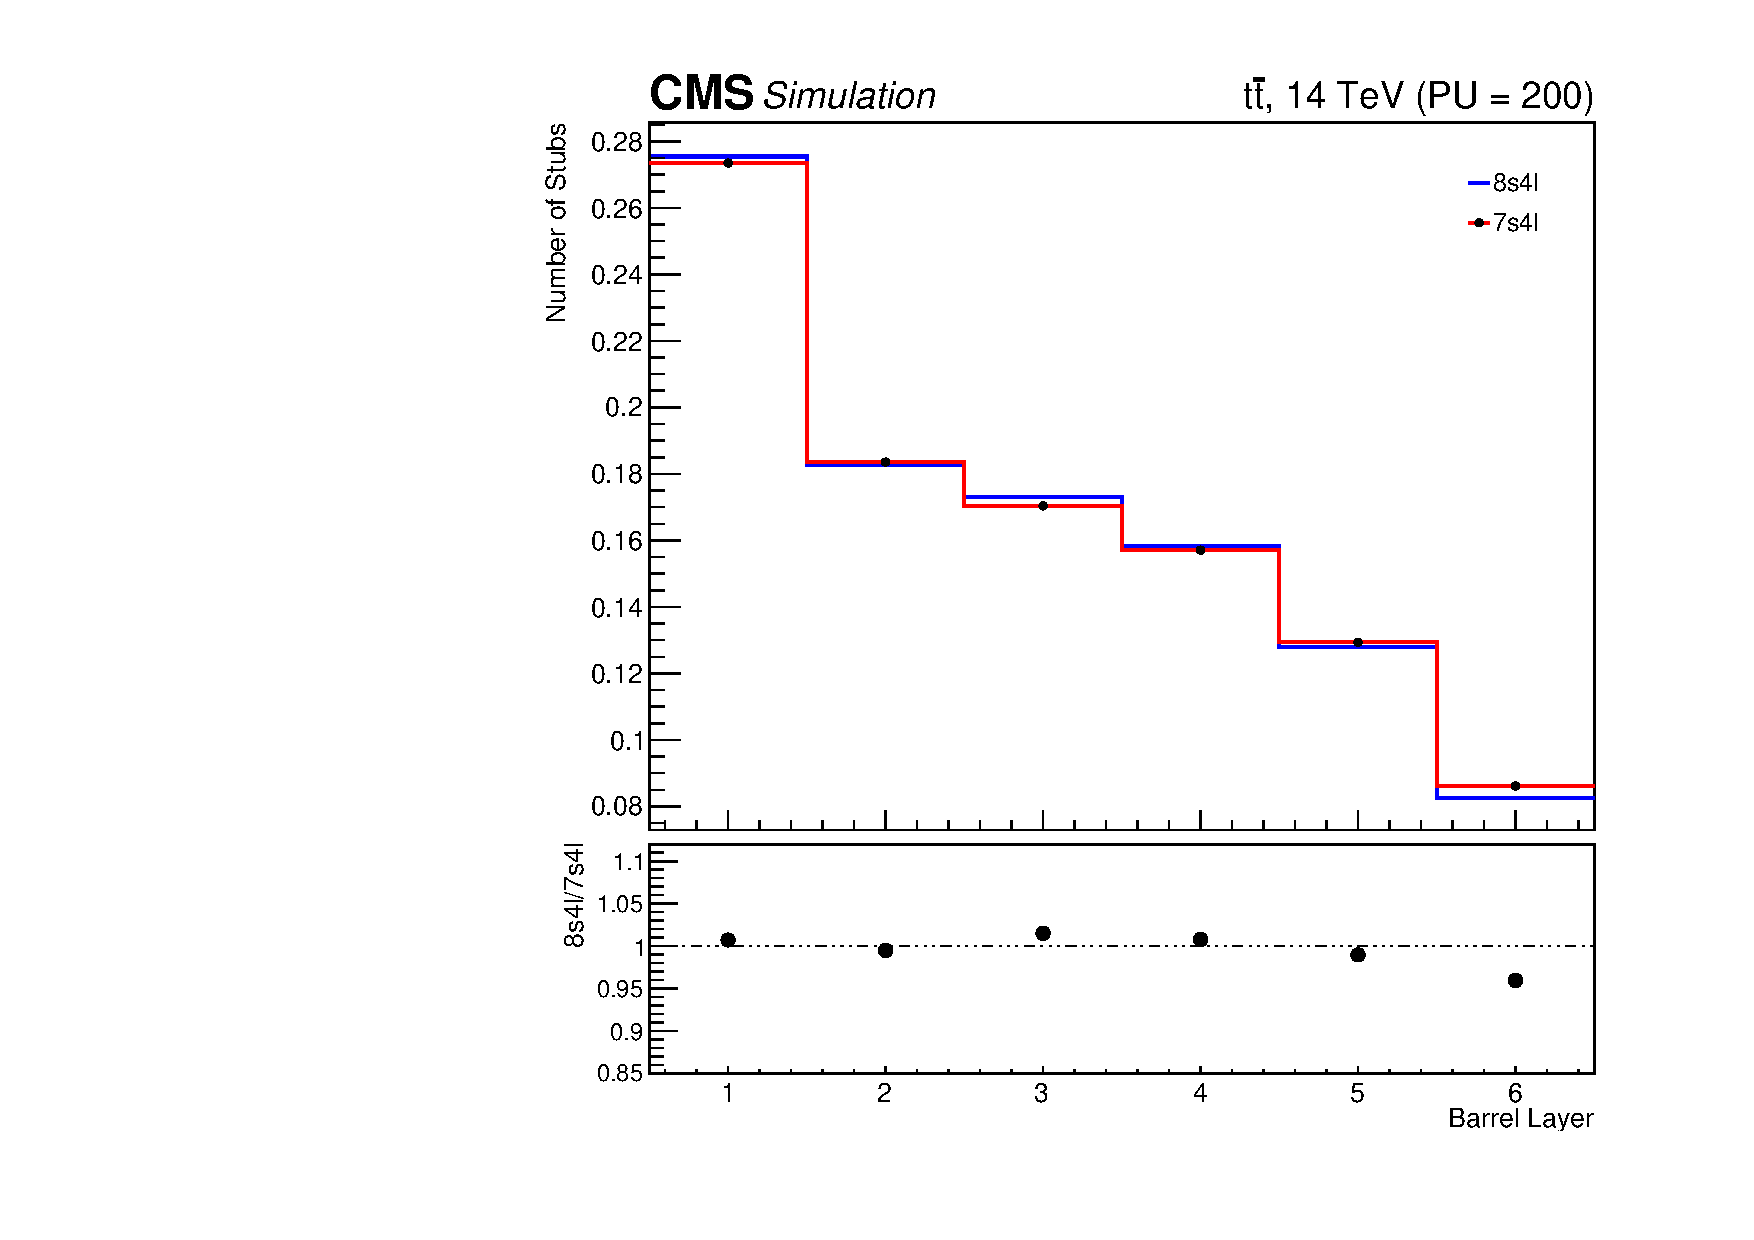
\includegraphics[width=0.32\textwidth]{NStubs_Barrel_8s4l_vs_7s4l_ratio.pdf}}
     \subfigure{
     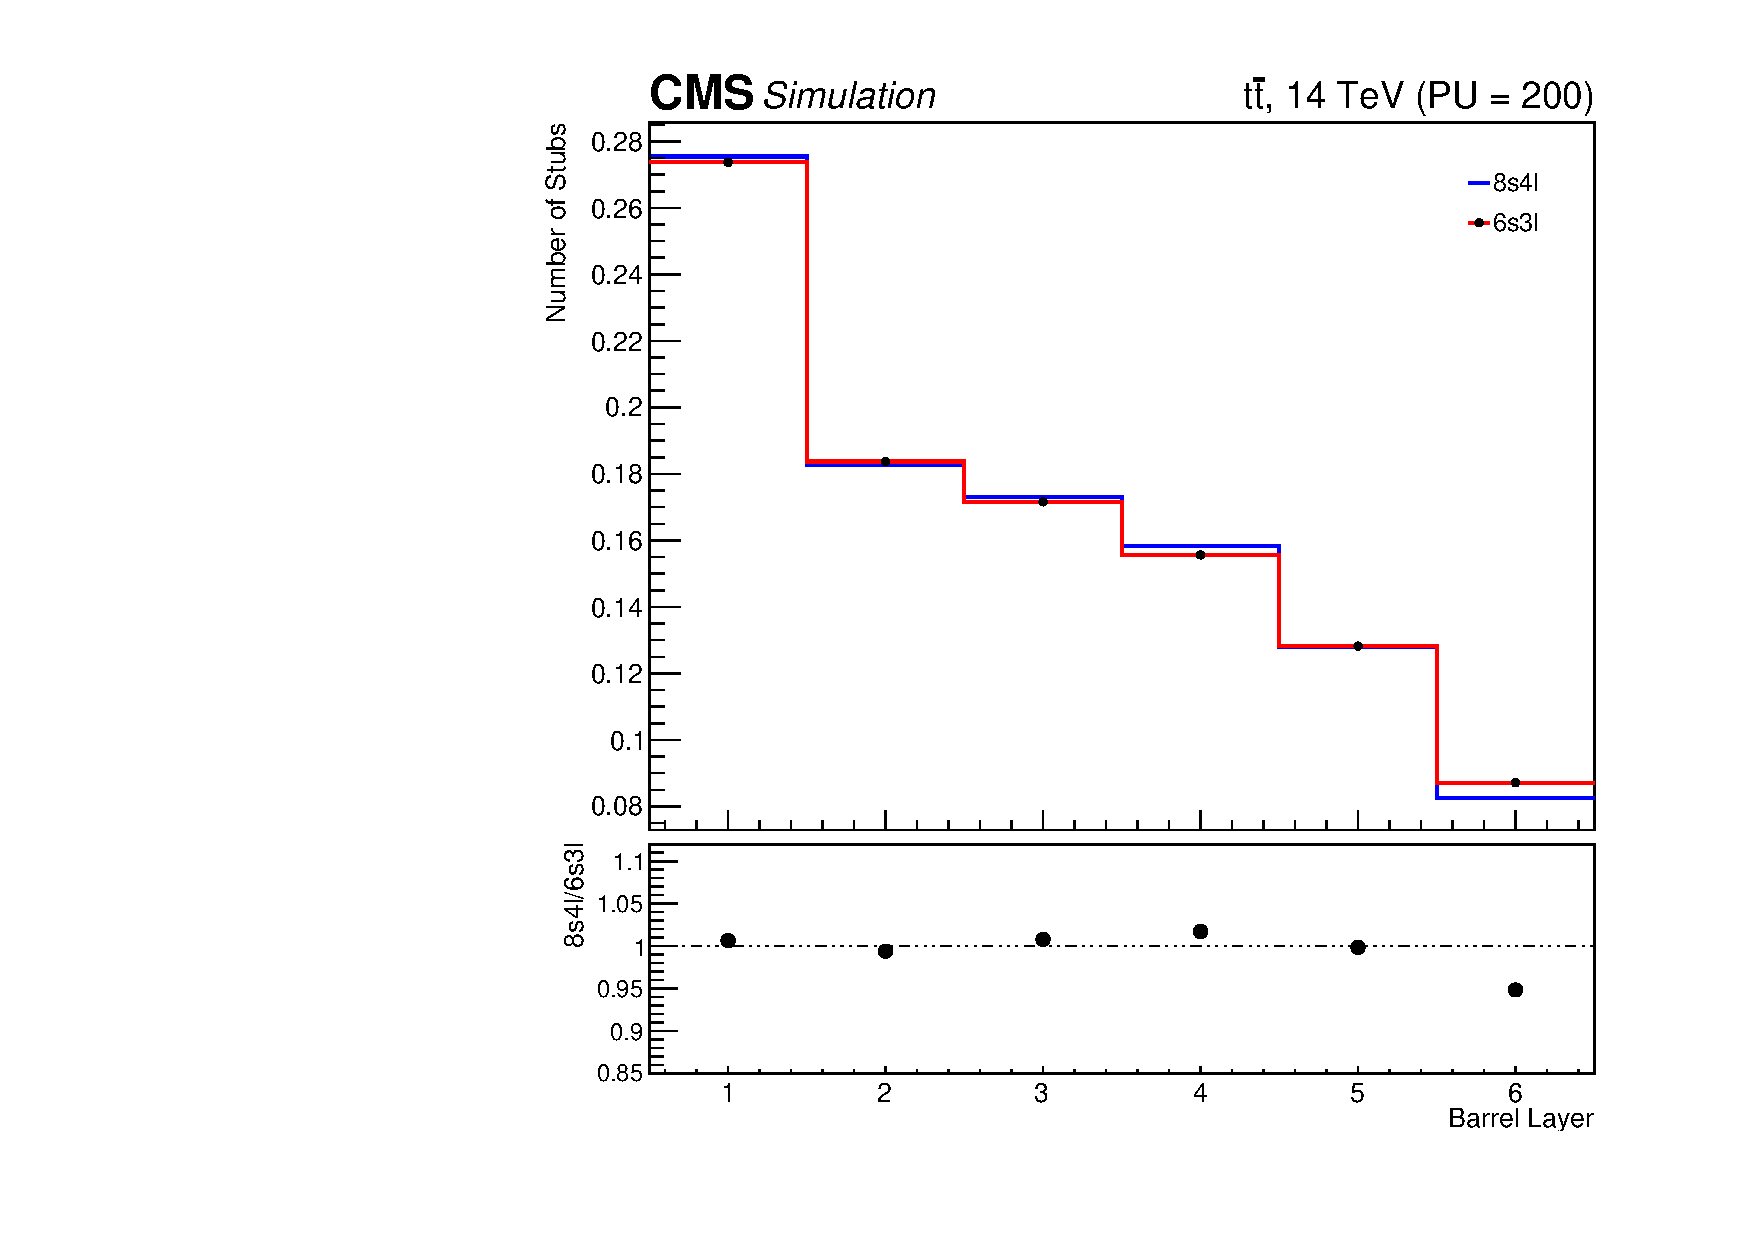
\includegraphics[width=0.32\textwidth]{NStubs_Barrel_8s4l_vs_6s3l_ratio.pdf}}
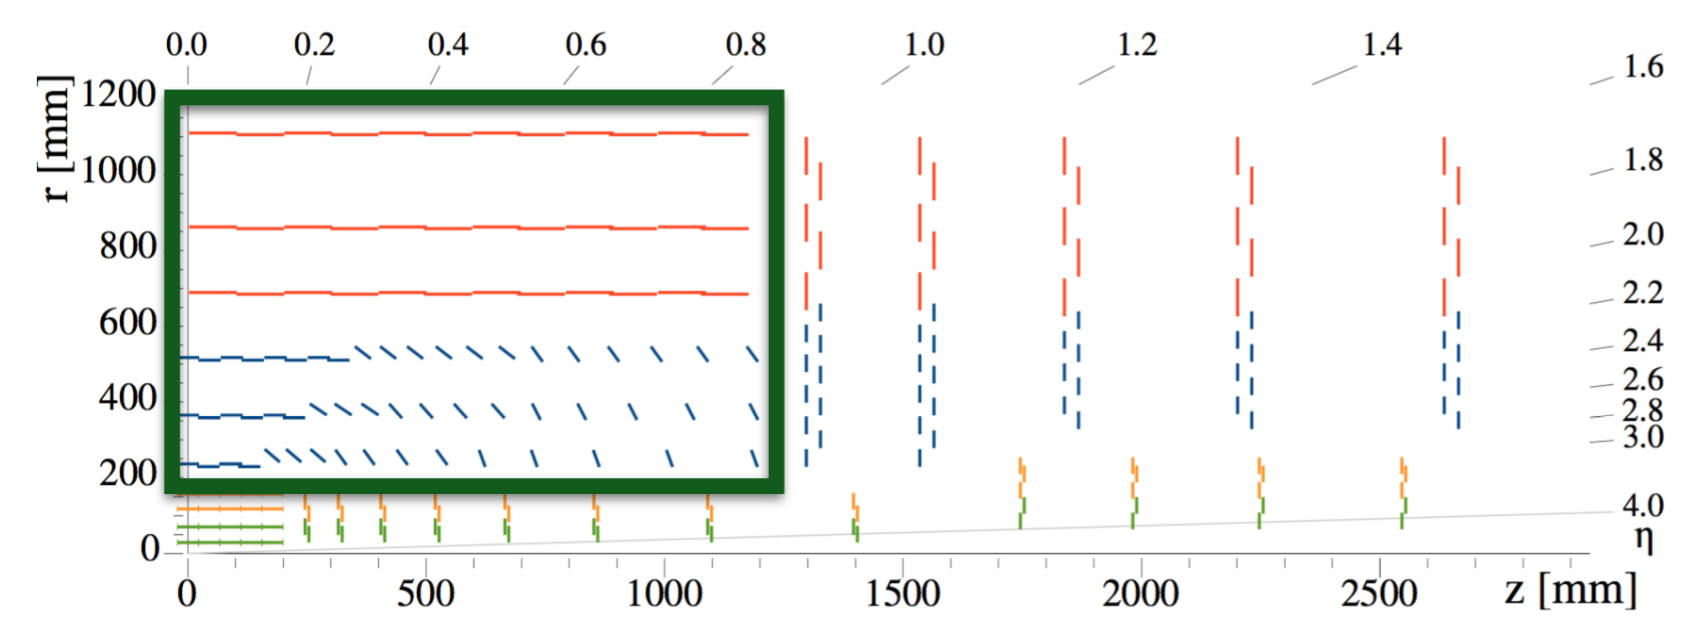
\includegraphics[width=0.8\textwidth]{TrackerBarrel.png}
  \caption{Comparison of total number of stubs per each of the 6 barrel layers. $8s4l$ vs $8s3l$ (left), $8s4l$ vs $7s4l$ (middle) and $8s4l$ vs $6s3l$ (right). Tracker Barrel layers shown below.}
\label{stubsBarrel}
\end{figure}

\begin{figure}[H]
    \centering
    \subfigure{
    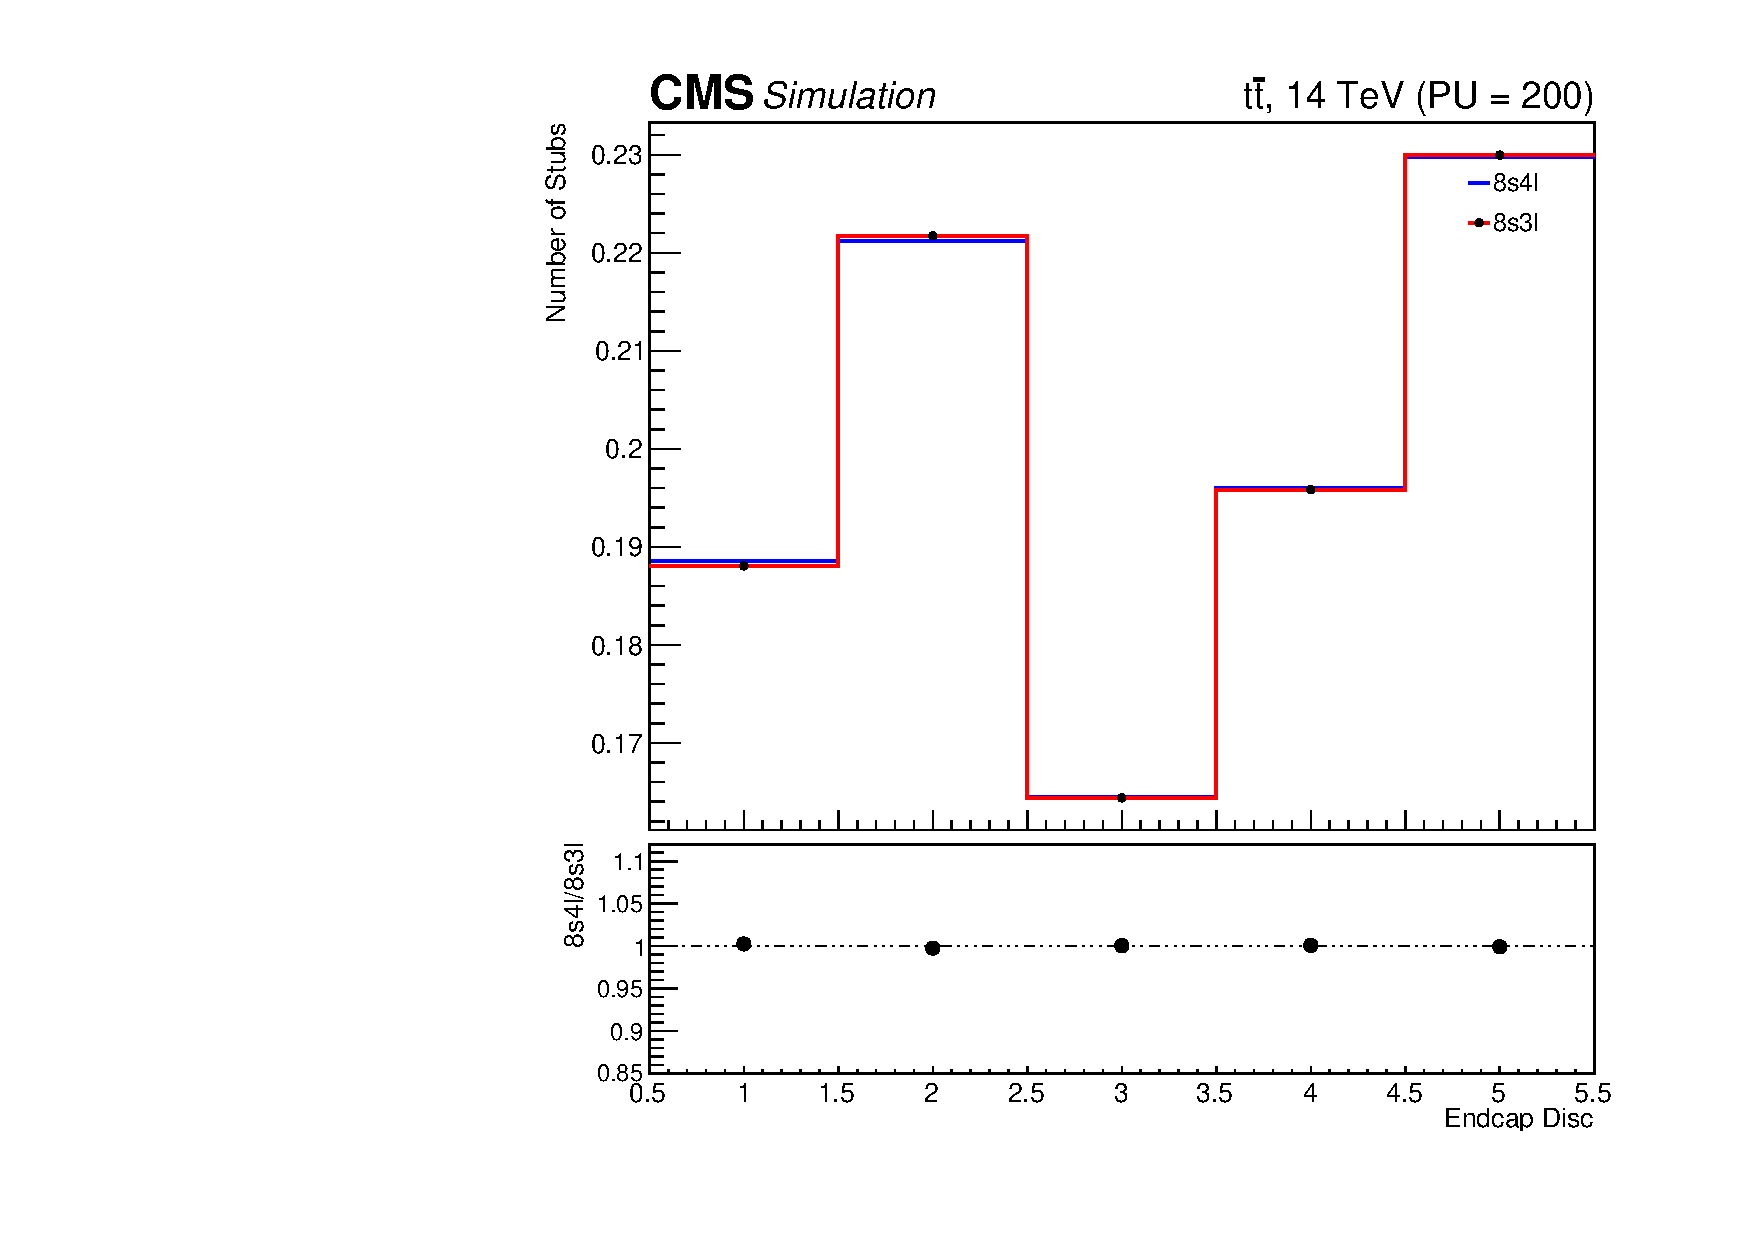
\includegraphics[width=0.32\textwidth]{NStubs_Endcap_Disc_8s4l_vs_8s3l_ratio.pdf}}
     \subfigure{
     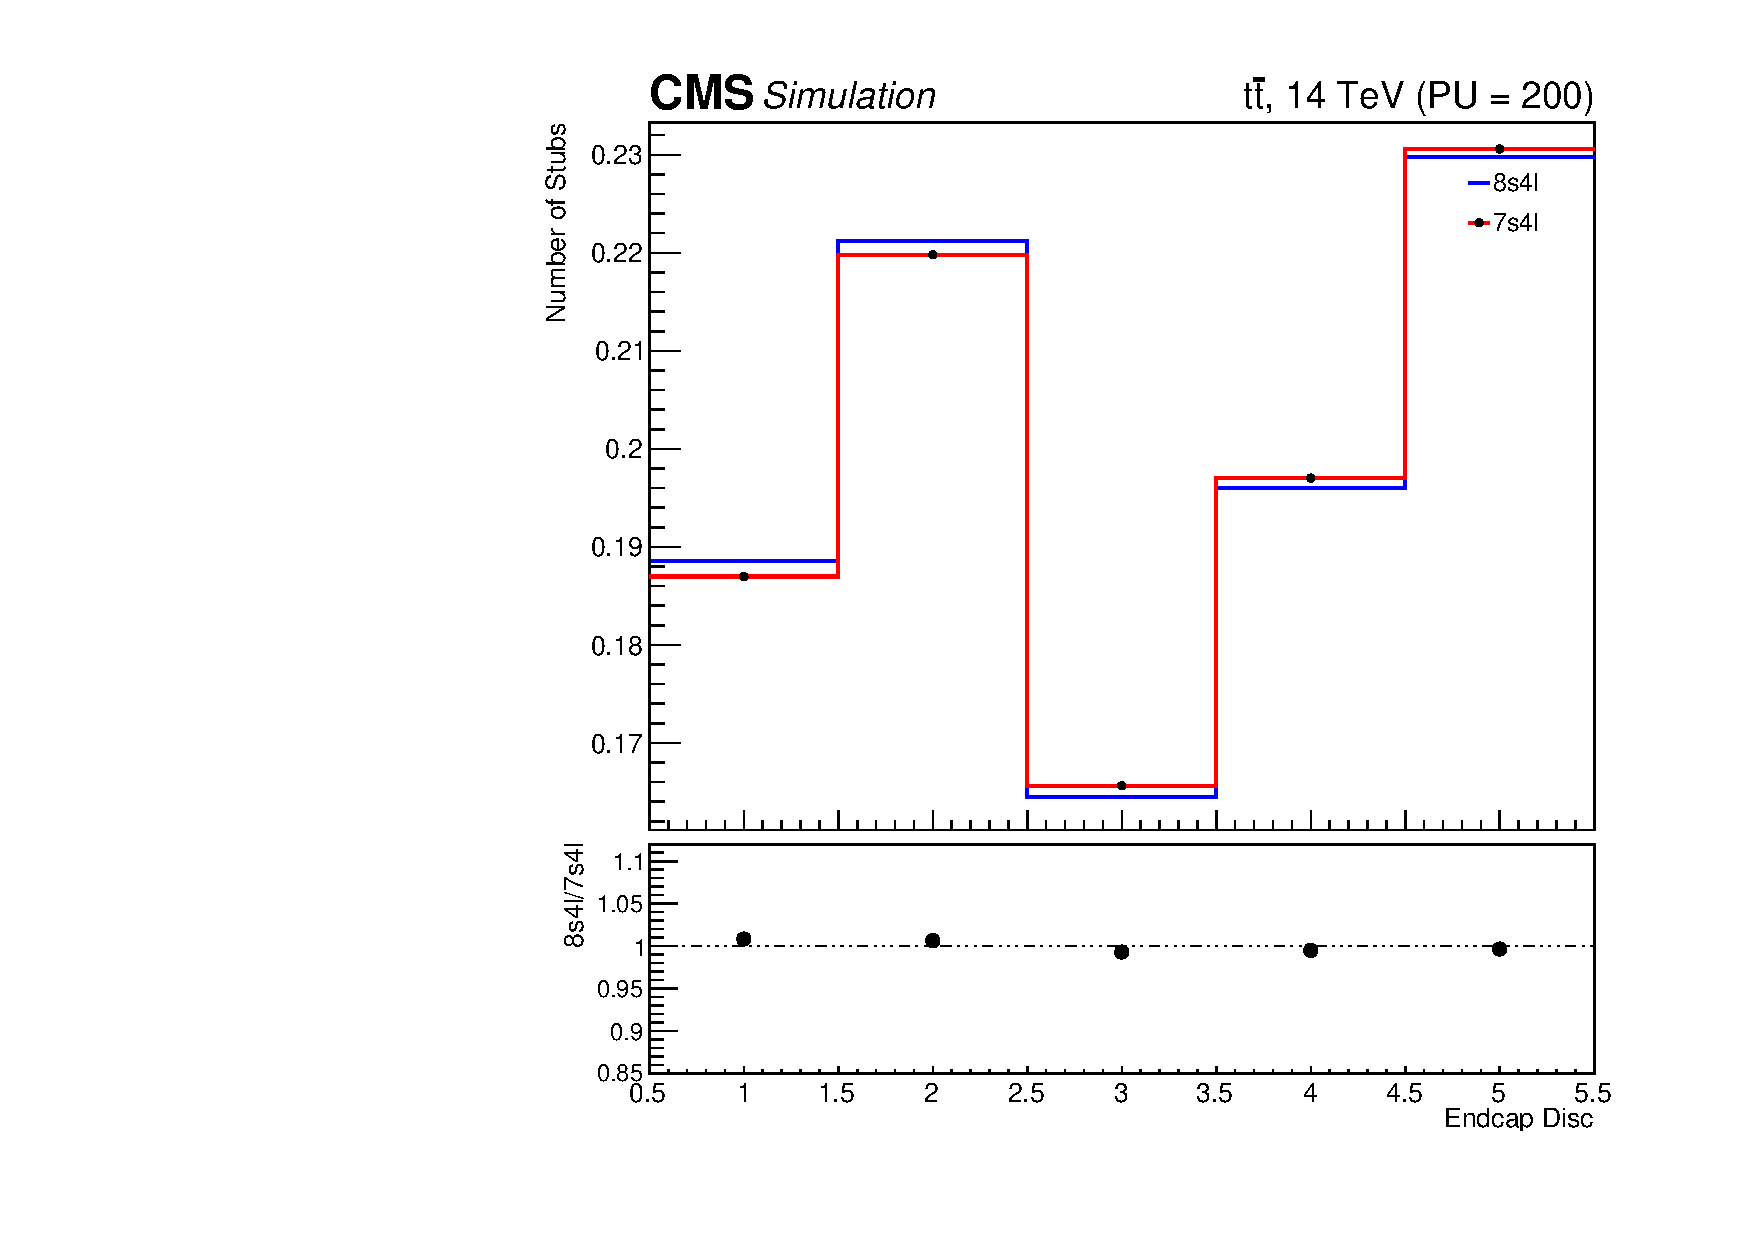
\includegraphics[width=0.32\textwidth]{NStubs_Endcap_Disc_8s4l_vs_7s4l_ratio.pdf}}
     \subfigure{
     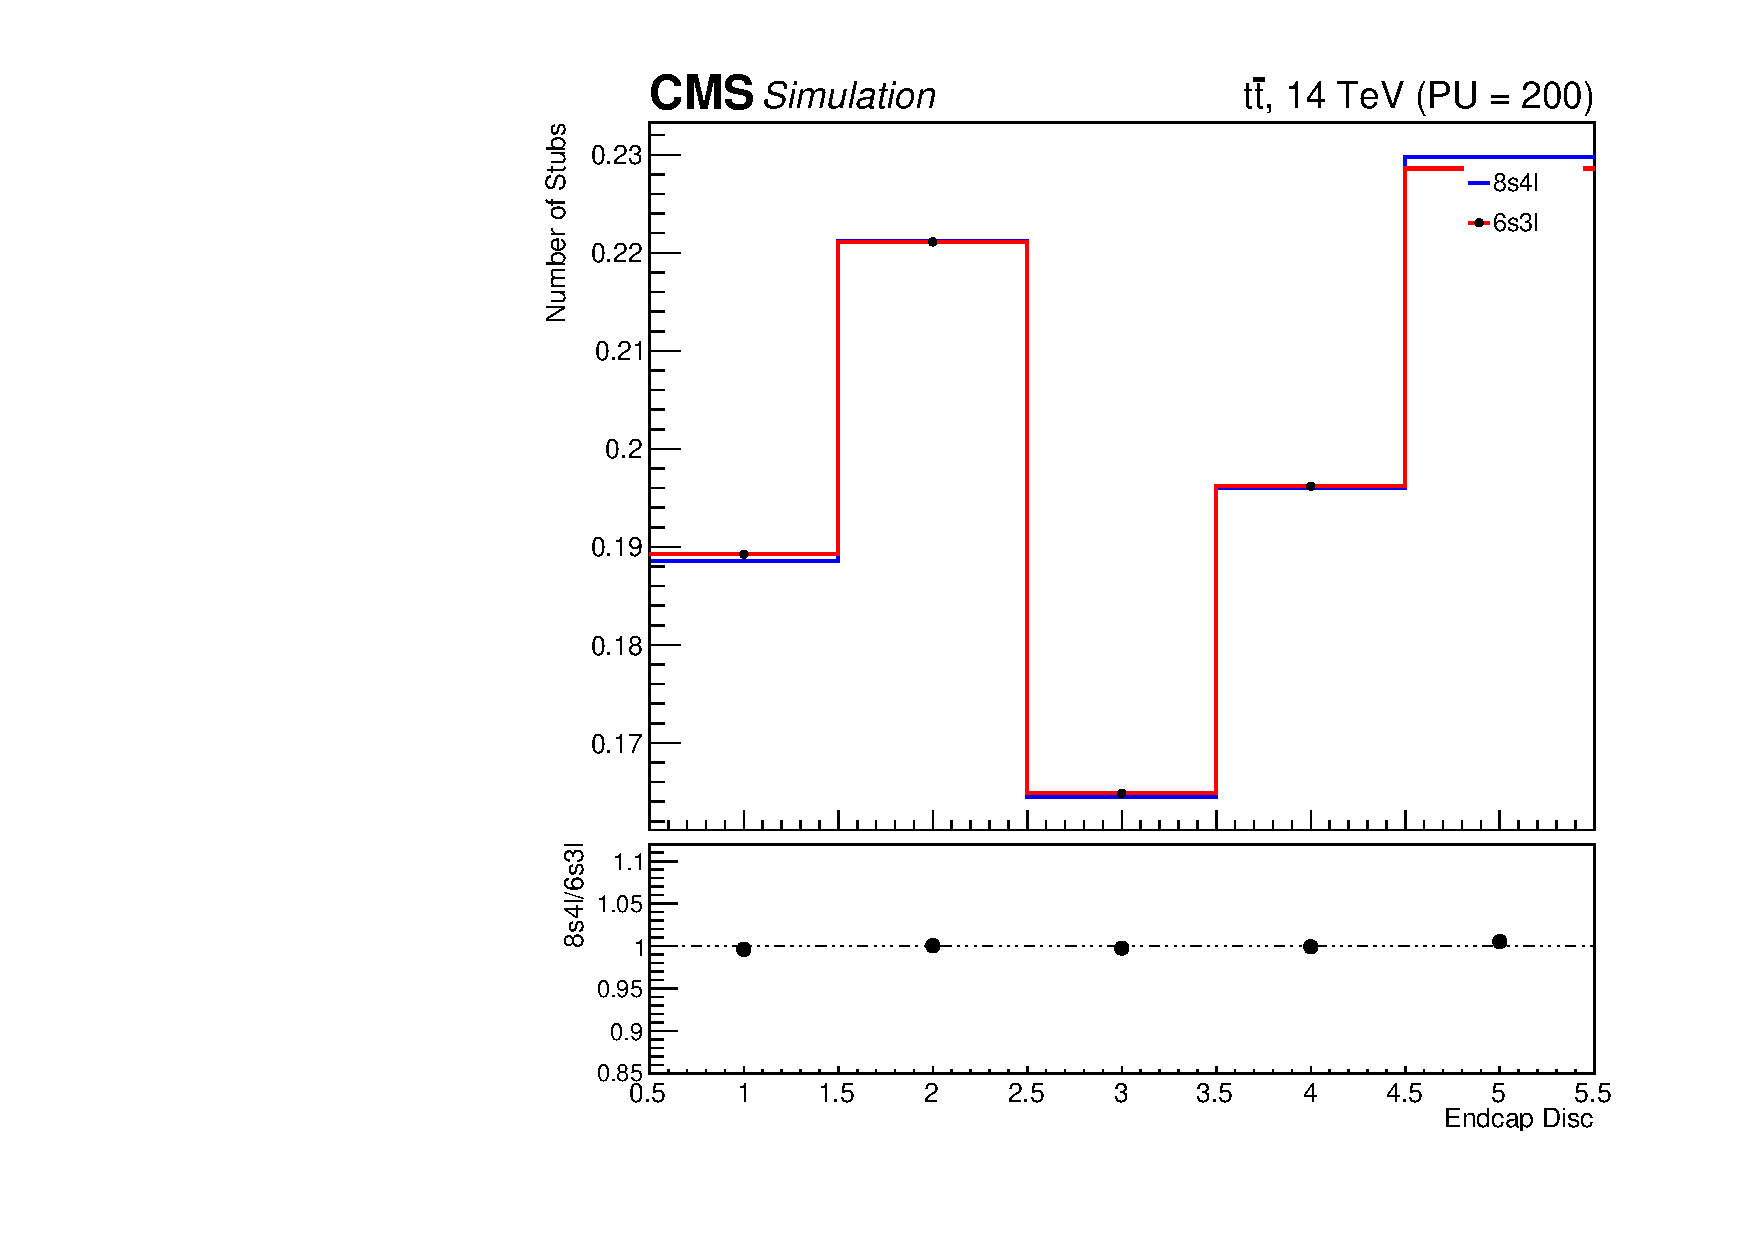
\includegraphics[width=0.32\textwidth]{NStubs_Endcap_Disc_8s4l_vs_6s3l_ratio.pdf}}
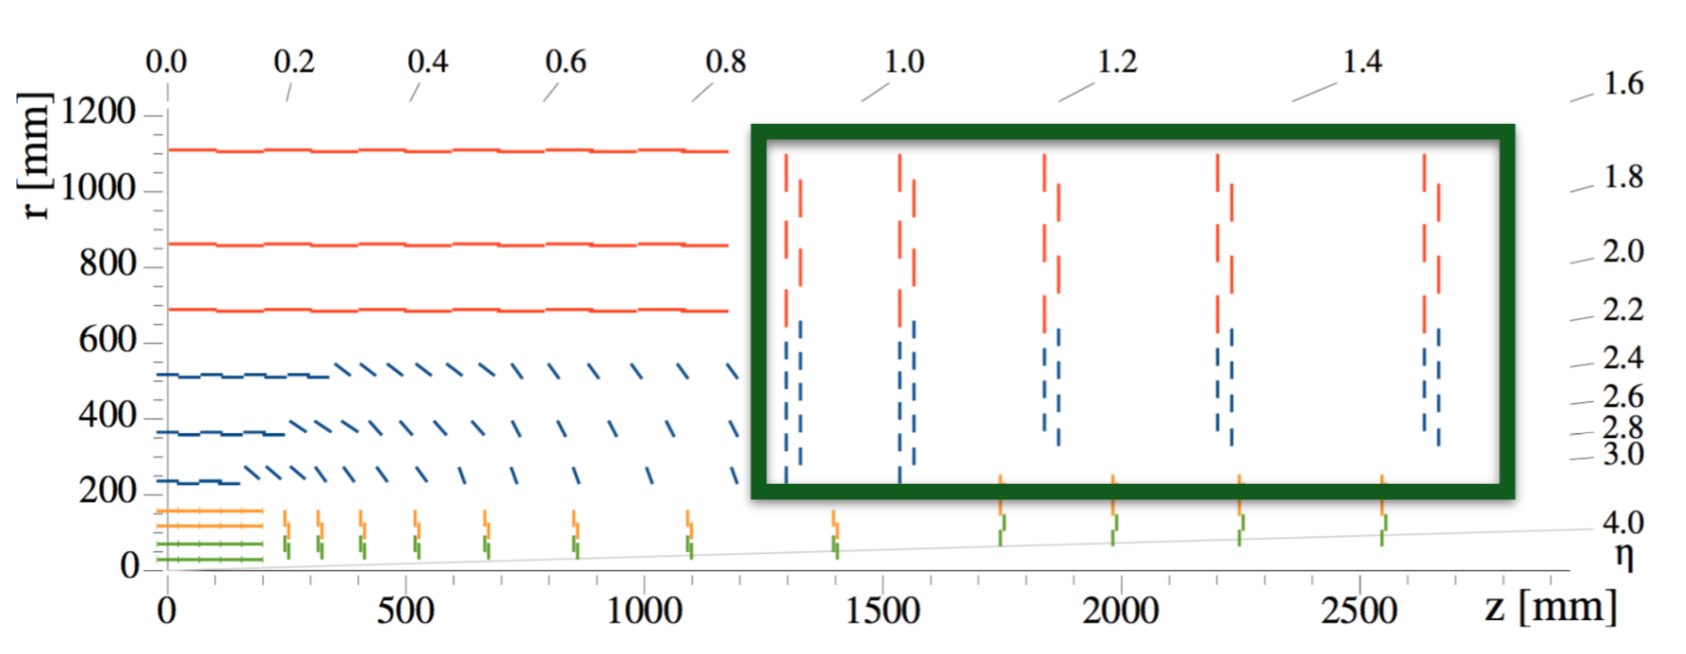
\includegraphics[width=0.8\textwidth]{TrackerEndcapDiscs.png}
  \caption{Comparison of total number of stubs per each of the 5 Endcap Double Discs. $8s4l$ vs $8s3l$ (left), $8s4l$ vs $7s4l$ (middle) and $8s4l$ vs $6s3l$ (right). Tracker Endcap Discs shown below.}\label{stubsEndcap}
\end{figure}

\begin{figure}[H]
    \centering
    \subfigure{
    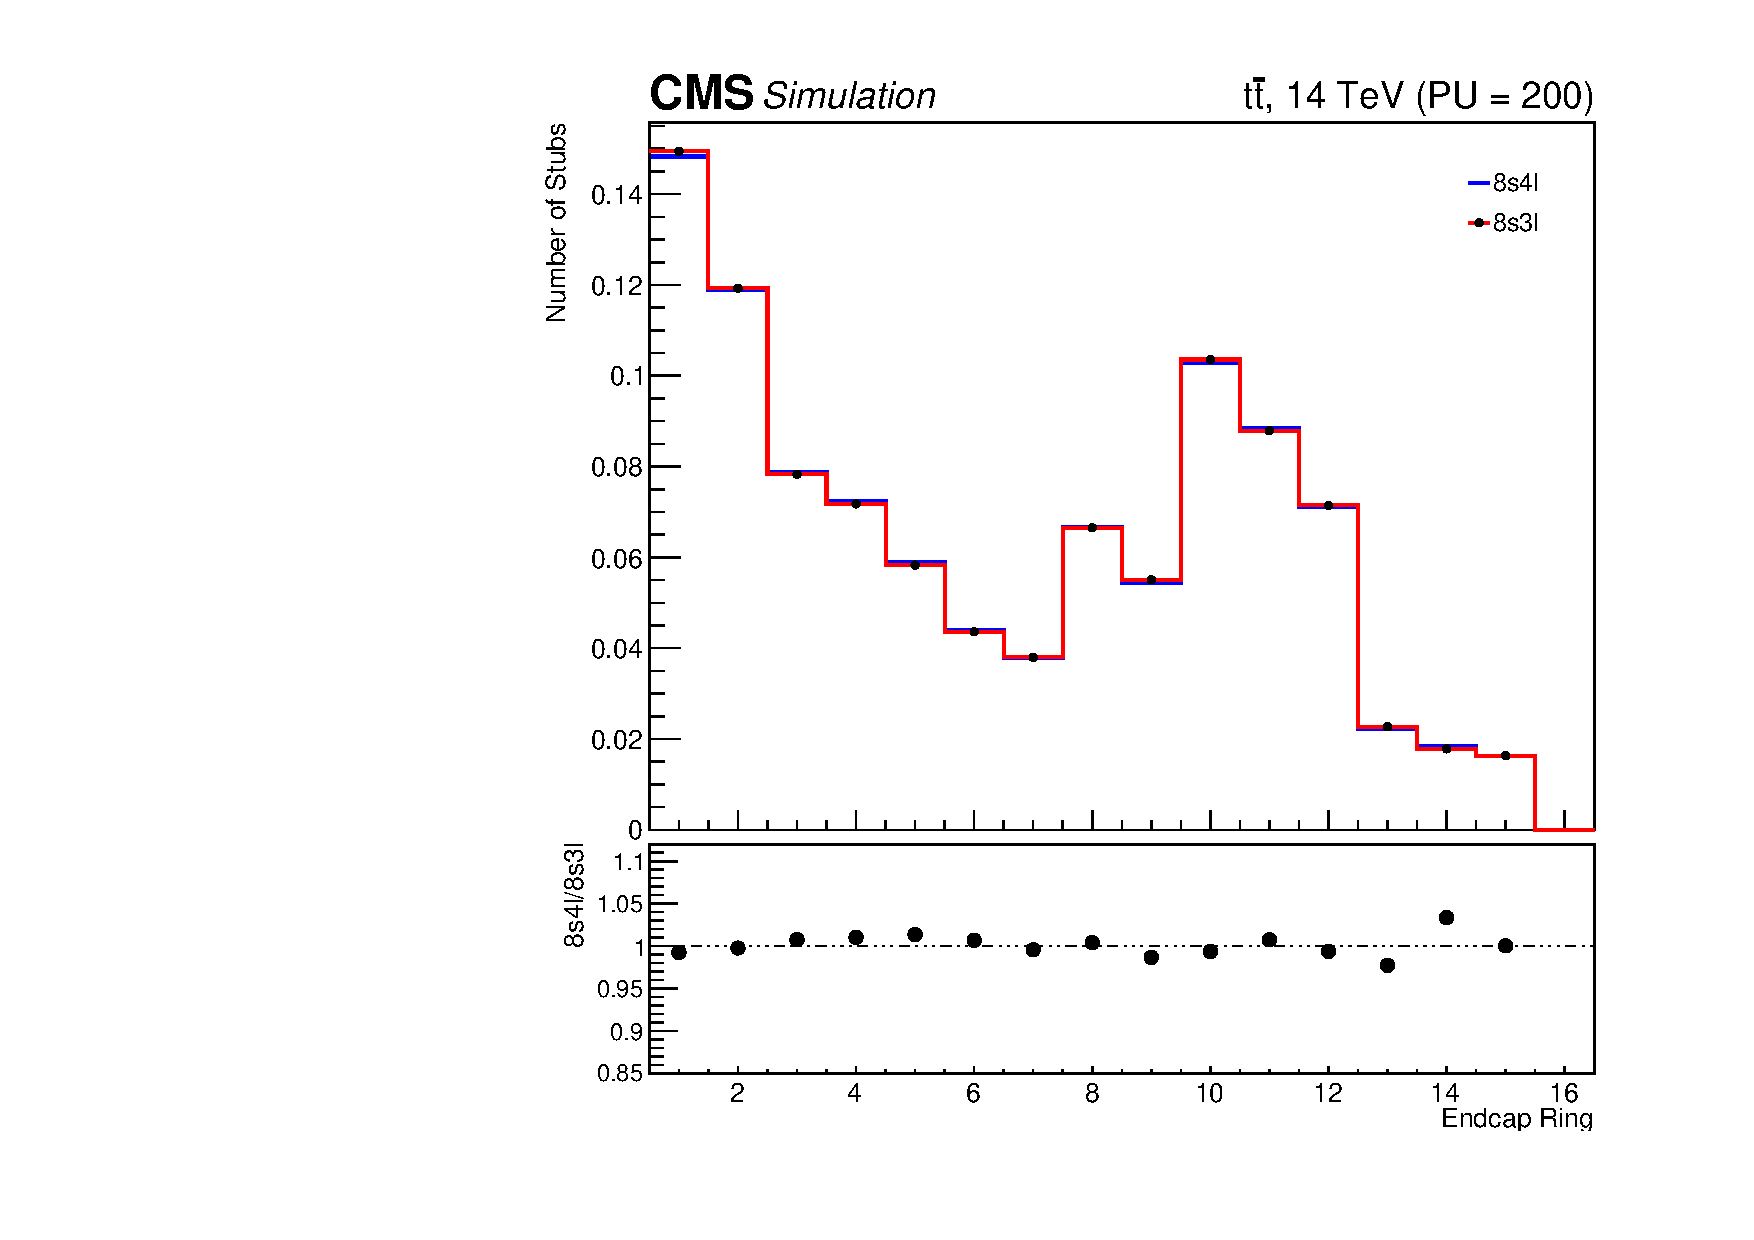
\includegraphics[width=0.32\textwidth]{NStubs_Endcap_Ring_8s4l_vs_8s3l_ratio.pdf}}
     \subfigure{
     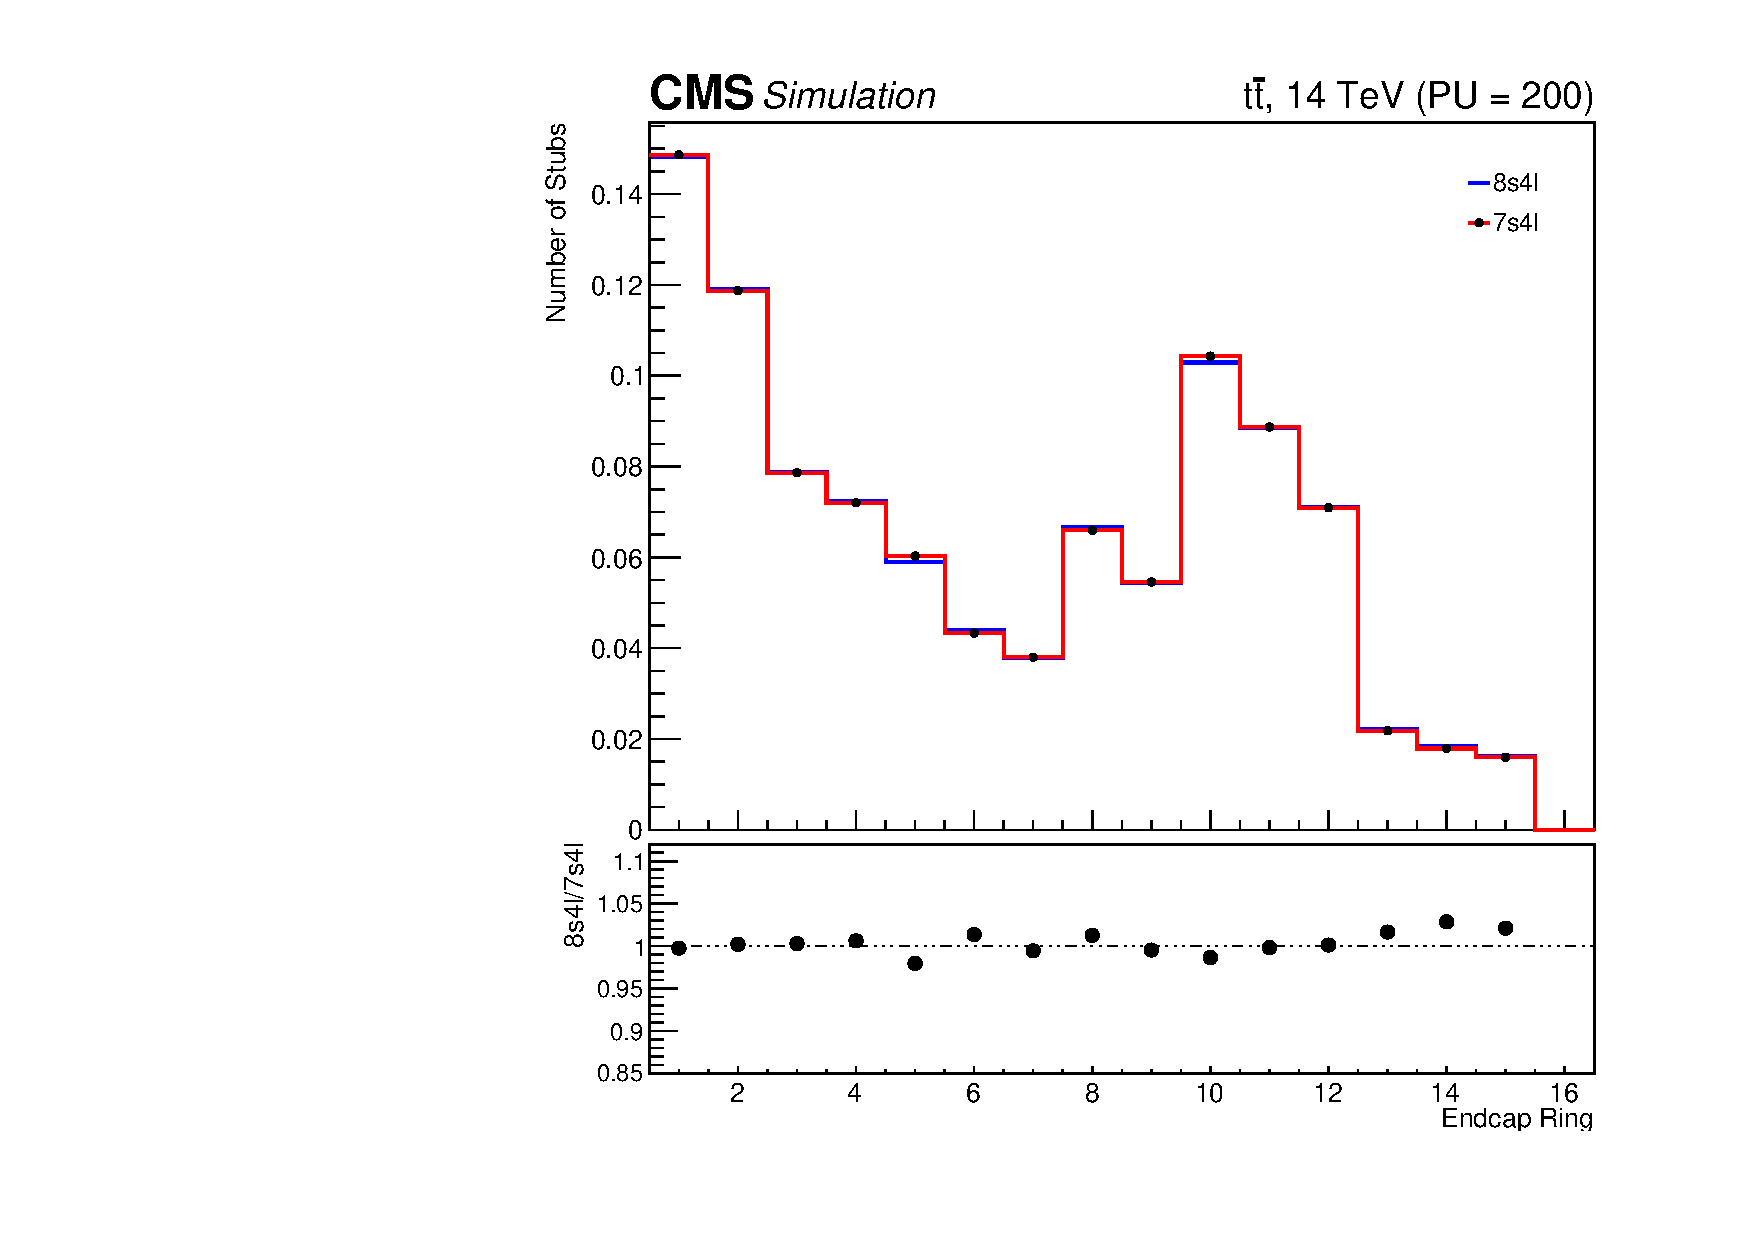
\includegraphics[width=0.32\textwidth]{NStubs_Endcap_Ring_8s4l_vs_7s4l_ratio.pdf}}
     \subfigure{
     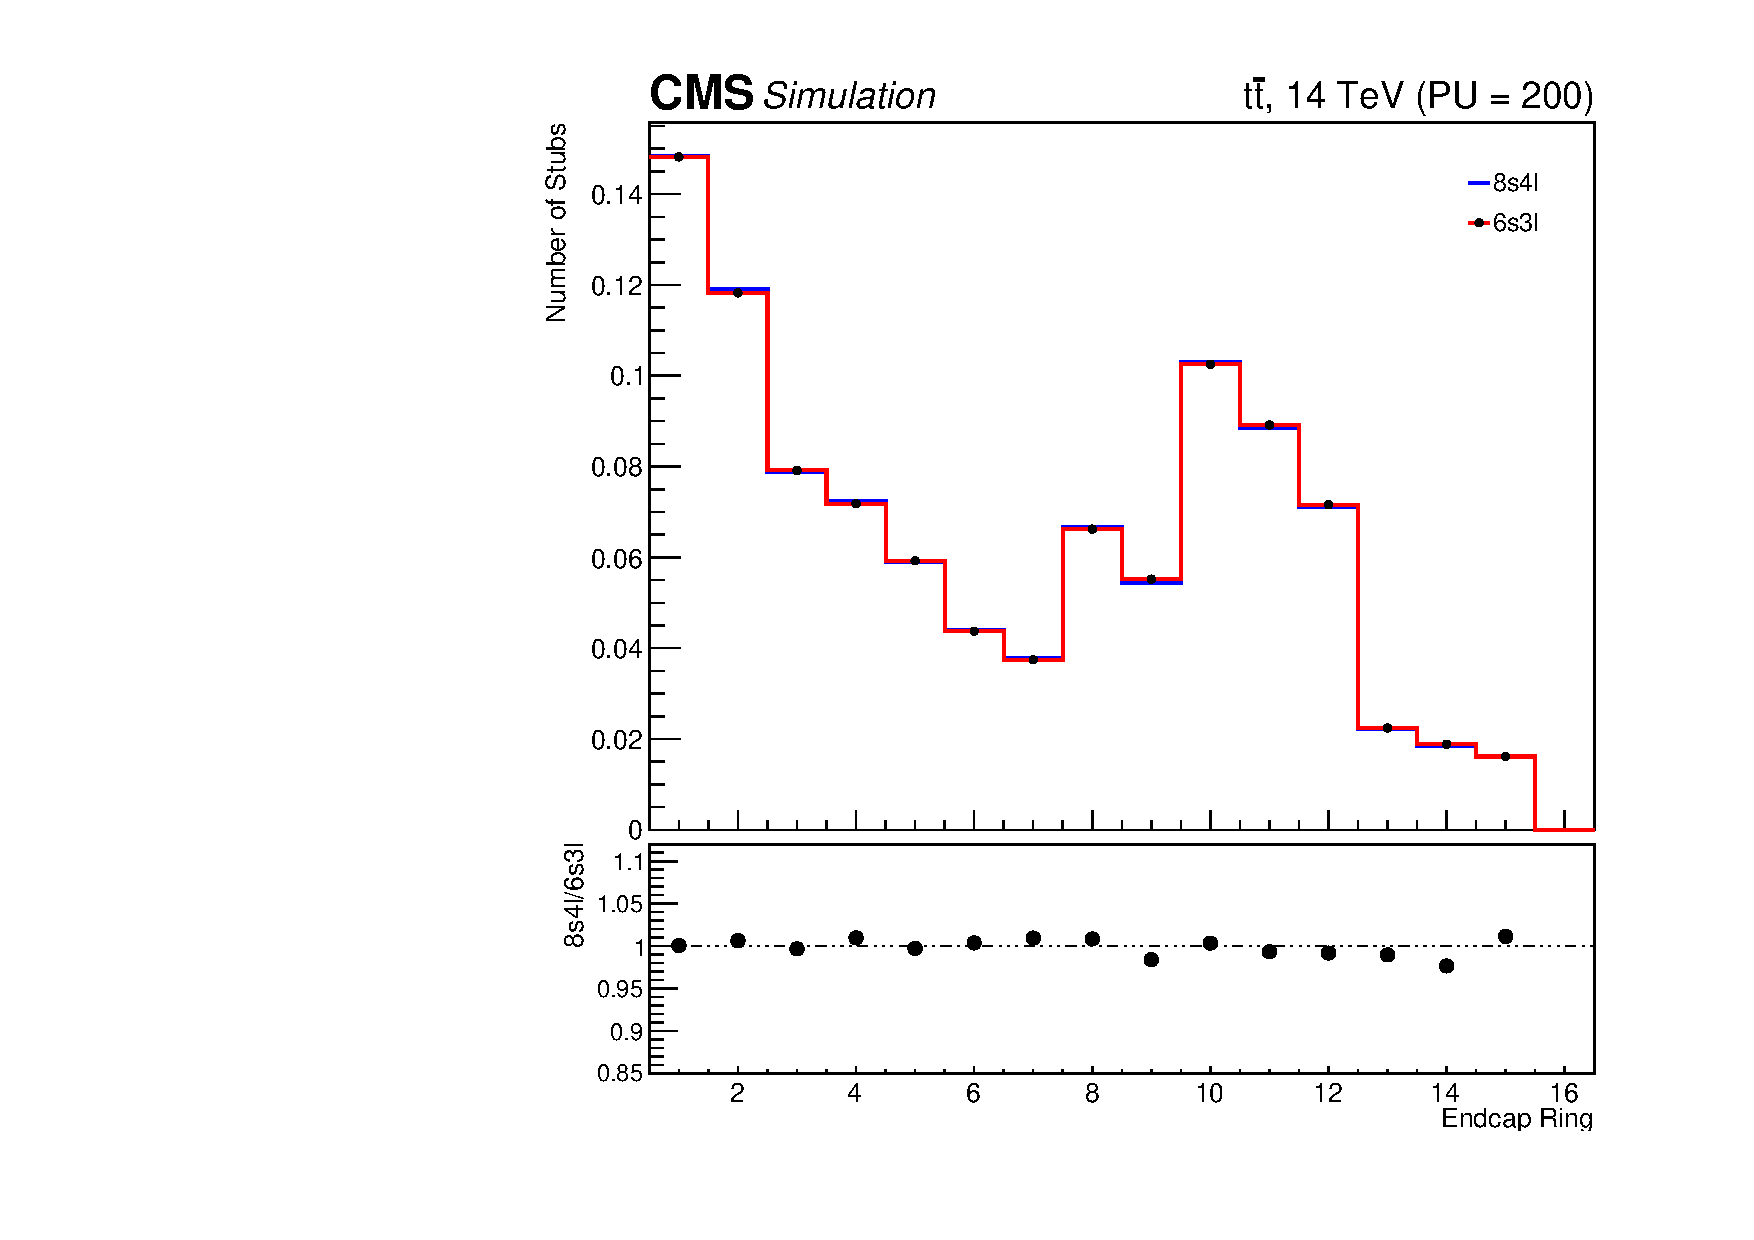
\includegraphics[width=0.32\textwidth]{NStubs_Endcap_Ring_8s4l_vs_6s3l_ratio.pdf}}
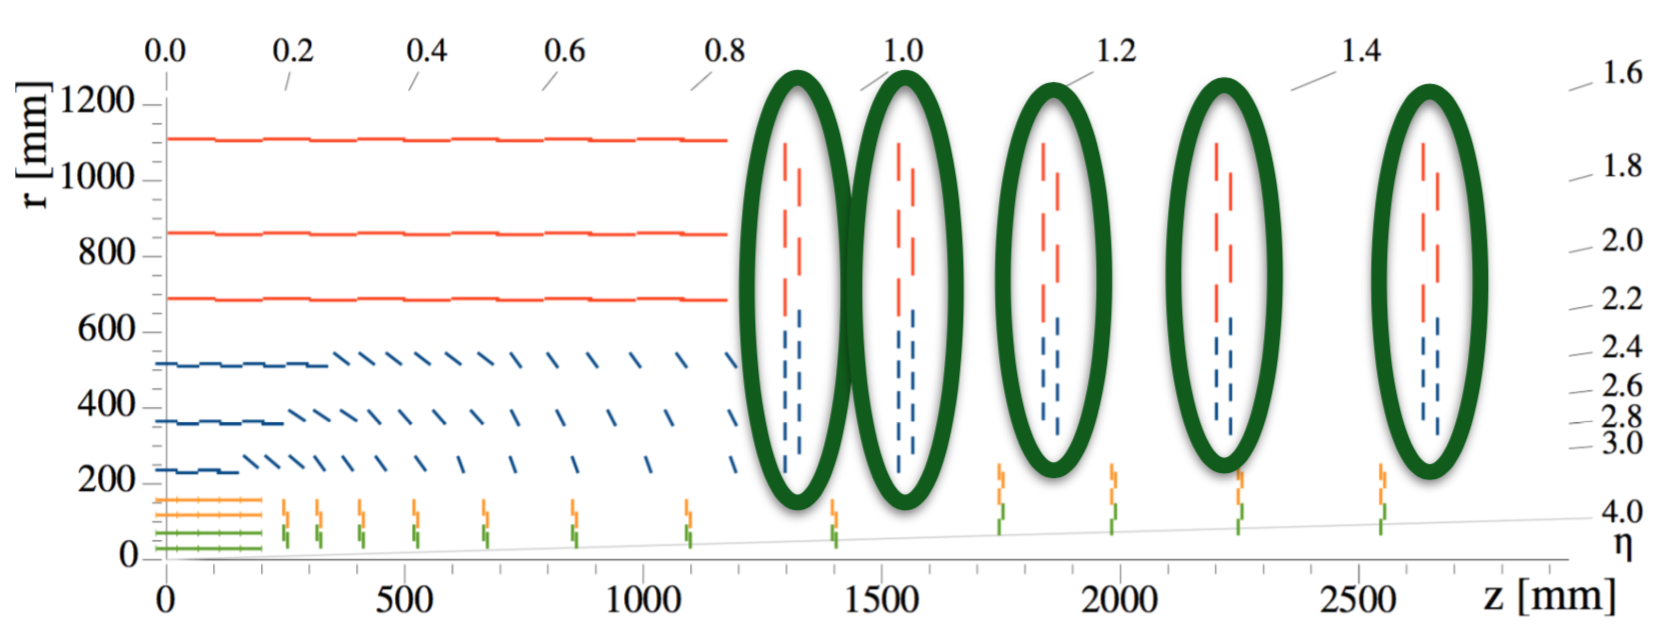
\includegraphics[width=0.8\textwidth]{AllDiscs.png}
  \caption{Comparison of total number of stubs for all rings across the five endcap double-discs. $8s4l$ vs $8s3l$ (left), $8s4l$ vs $7s4l$ (middle) and $8s4l$ vs $6s3l$ (right). The double discs are shown below.}
\label{stubsPerRing}
\end{figure}

\vspace{1em}

\section{Results}

The above study shows that the removal of discs in the pixel detector affects the number of stubs formed in the OT. A reduction in the amount of material (i.e. removal of discs) translates into a reduced amount of secondary particle interactions and hence, a decrease in the net amount of stubs is observed. In other words more material (more discs) in the pixel layer leads to more secondaries, increasing the total amount of stubs in a given sample. However, the effect is small and a detailed study with respect to various $\eta$ regions is planned in the future, as stub formation is also sensitive to $\eta$ windows. Knowing the origin of particles causing stubs is also an important area to look into.

